\documentclass[1p]{elsarticle_modified}
%\bibliographystyle{elsarticle-num}

%\usepackage[colorlinks]{hyperref}
%\usepackage{abbrmath_seonhwa} %\Abb, \Ascr, \Acal ,\Abf, \Afrak
\usepackage{amsfonts}
\usepackage{amssymb}
\usepackage{amsmath}
\usepackage{amsthm}
\usepackage{scalefnt}
\usepackage{amsbsy}
\usepackage{kotex}
\usepackage{caption}
\usepackage{subfig}
\usepackage{color}
\usepackage{graphicx}
\usepackage{xcolor} %% white, black, red, green, blue, cyan, magenta, yellow
\usepackage{float}
\usepackage{setspace}
\usepackage{hyperref}

\usepackage{tikz}
\usetikzlibrary{arrows}

\usepackage{multirow}
\usepackage{array} % fixed length table
\usepackage{hhline}

%%%%%%%%%%%%%%%%%%%%%
\makeatletter
\renewcommand*\env@matrix[1][\arraystretch]{%
	\edef\arraystretch{#1}%
	\hskip -\arraycolsep
	\let\@ifnextchar\new@ifnextchar
	\array{*\c@MaxMatrixCols c}}
\makeatother %https://tex.stackexchange.com/questions/14071/how-can-i-increase-the-line-spacing-in-a-matrix
%%%%%%%%%%%%%%%

\usepackage[normalem]{ulem}

\newcommand{\msout}[1]{\ifmmode\text{\sout{\ensuremath{#1}}}\else\sout{#1}\fi}
%SOURCE: \msout is \stkout macro in https://tex.stackexchange.com/questions/20609/strikeout-in-math-mode

\newcommand{\cancel}[1]{
	\ifmmode
	{\color{red}\msout{#1}}
	\else
	{\color{red}\sout{#1}}
	\fi
}

\newcommand{\add}[1]{
	{\color{blue}\uwave{#1}}
}

\newcommand{\replace}[2]{
	\ifmmode
	{\color{red}\msout{#1}}{\color{blue}\uwave{#2}}
	\else
	{\color{red}\sout{#1}}{\color{blue}\uwave{#2}}
	\fi
}

\newcommand{\Sol}{\mathcal{S}} %segment
\newcommand{\D}{D} %diagram
\newcommand{\A}{\mathcal{A}} %arc


%%%%%%%%%%%%%%%%%%%%%%%%%%%%%5 test

\def\sl{\operatorname{\textup{SL}}(2,\Cbb)}
\def\psl{\operatorname{\textup{PSL}}(2,\Cbb)}
\def\quan{\mkern 1mu \triangleright \mkern 1mu}

\theoremstyle{definition}
\newtheorem{thm}{Theorem}[section]
\newtheorem{prop}[thm]{Proposition}
\newtheorem{lem}[thm]{Lemma}
\newtheorem{ques}[thm]{Question}
\newtheorem{cor}[thm]{Corollary}
\newtheorem{defn}[thm]{Definition}
\newtheorem{exam}[thm]{Example}
\newtheorem{rmk}[thm]{Remark}
\newtheorem{alg}[thm]{Algorithm}

\newcommand{\I}{\sqrt{-1}}
\begin{document}

%\begin{frontmatter}
%
%\title{Boundary parabolic representations of knots up to 8 crossings}
%
%%% Group authors per affiliation:
%\author{Yunhi Cho} 
%\address{Department of Mathematics, University of Seoul, Seoul, Korea}
%\ead{yhcho@uos.ac.kr}
%
%
%\author{Seonhwa Kim} %\fnref{s_kim}}
%\address{Center for Geometry and Physics, Institute for Basic Science, Pohang, 37673, Korea}
%\ead{ryeona17@ibs.re.kr}
%
%\author{Hyuk Kim}
%\address{Department of Mathematical Sciences, Seoul National University, Seoul 08826, Korea}
%\ead{hyukkim@snu.ac.kr}
%
%\author{Seokbeom Yoon}
%\address{Department of Mathematical Sciences, Seoul National University, Seoul, 08826,  Korea}
%\ead{sbyoon15@snu.ac.kr}
%
%\begin{abstract}
%We find all boundary parabolic representation of knots up to 8 crossings.
%
%\end{abstract}
%\begin{keyword}
%    \MSC[2010] 57M25 
%\end{keyword}
%
%\end{frontmatter}

%\linenumbers
%\tableofcontents
%
\newcommand\colored[1]{\textcolor{white}{\rule[-0.35ex]{0.8em}{1.4ex}}\kern-0.8em\color{red} #1}%
%\newcommand\colored[1]{\textcolor{white}{ #1}\kern-2.17ex	\textcolor{white}{ #1}\kern-1.81ex	\textcolor{white}{ #1}\kern-2.15ex\color{red}#1	}

{\Large $\underline{12a_{0973}~(K12a_{0973})}$}

\setlength{\tabcolsep}{10pt}
\renewcommand{\arraystretch}{1.6}
\vspace{1cm}\begin{tabular}{m{100pt}>{\centering\arraybackslash}m{274pt}}
\multirow{5}{120pt}{
	\centering
	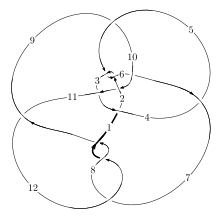
\includegraphics[width=112pt]{../../../GIT/diagram.site/Diagrams/png/1774_12a_0973.png}\\
\ \ \ A knot diagram\footnotemark}&
\allowdisplaybreaks
\textbf{Linearized knot diagam} \\
\cline{2-2}
 &
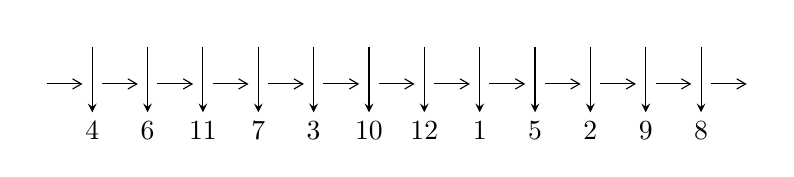
\begin{tikzpicture}[x=20pt, y=17pt]
	% nodes
	\node (C0) at (0, 0) {};
	\node (C1) at (1, 0) {};
	\node (C1U) at (1, +1) {};
	\node (C1D) at (1, -1) {4};

	\node (C2) at (2, 0) {};
	\node (C2U) at (2, +1) {};
	\node (C2D) at (2, -1) {6};

	\node (C3) at (3, 0) {};
	\node (C3U) at (3, +1) {};
	\node (C3D) at (3, -1) {11};

	\node (C4) at (4, 0) {};
	\node (C4U) at (4, +1) {};
	\node (C4D) at (4, -1) {7};

	\node (C5) at (5, 0) {};
	\node (C5U) at (5, +1) {};
	\node (C5D) at (5, -1) {3};

	\node (C6) at (6, 0) {};
	\node (C6U) at (6, +1) {};
	\node (C6D) at (6, -1) {10};

	\node (C7) at (7, 0) {};
	\node (C7U) at (7, +1) {};
	\node (C7D) at (7, -1) {12};

	\node (C8) at (8, 0) {};
	\node (C8U) at (8, +1) {};
	\node (C8D) at (8, -1) {1};

	\node (C9) at (9, 0) {};
	\node (C9U) at (9, +1) {};
	\node (C9D) at (9, -1) {5};

	\node (C10) at (10, 0) {};
	\node (C10U) at (10, +1) {};
	\node (C10D) at (10, -1) {2};

	\node (C11) at (11, 0) {};
	\node (C11U) at (11, +1) {};
	\node (C11D) at (11, -1) {9};

	\node (C12) at (12, 0) {};
	\node (C12U) at (12, +1) {};
	\node (C12D) at (12, -1) {8};
	\node (C13) at (13, 0) {};

	% arrows
	\draw[->,>={angle 60}]
	(C0) edge (C1) (C1) edge (C2) (C2) edge (C3) (C3) edge (C4) (C4) edge (C5) (C5) edge (C6) (C6) edge (C7) (C7) edge (C8) (C8) edge (C9) (C9) edge (C10) (C10) edge (C11) (C11) edge (C12) (C12) edge (C13) ;	\draw[->,>=stealth]
	(C1U) edge (C1D) (C2U) edge (C2D) (C3U) edge (C3D) (C4U) edge (C4D) (C5U) edge (C5D) (C6U) edge (C6D) (C7U) edge (C7D) (C8U) edge (C8D) (C9U) edge (C9D) (C10U) edge (C10D) (C11U) edge (C11D) (C12U) edge (C12D) ;
	\end{tikzpicture} \\
\hhline{~~} \\& 
\textbf{Solving Sequence} \\ \cline{2-2} 
 &
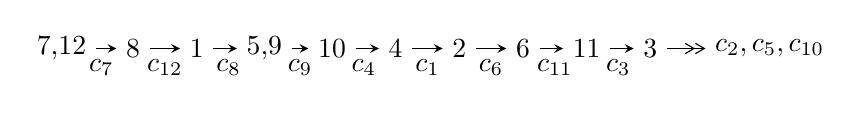
\begin{tikzpicture}[x=23pt, y=7pt]
	% node
	\node (A0) at (-1/8, 0) {7,12};
	\node (A1) at (1, 0) {8};
	\node (A2) at (2, 0) {1};
	\node (A3) at (49/16, 0) {5,9};
	\node (A4) at (33/8, 0) {10};
	\node (A5) at (41/8, 0) {4};
	\node (A6) at (49/8, 0) {2};
	\node (A7) at (57/8, 0) {6};
	\node (A8) at (65/8, 0) {11};
	\node (A9) at (73/8, 0) {3};
	\node (C1) at (1/2, -1) {$c_{7}$};
	\node (C2) at (3/2, -1) {$c_{12}$};
	\node (C3) at (5/2, -1) {$c_{8}$};
	\node (C4) at (29/8, -1) {$c_{9}$};
	\node (C5) at (37/8, -1) {$c_{4}$};
	\node (C6) at (45/8, -1) {$c_{1}$};
	\node (C7) at (53/8, -1) {$c_{6}$};
	\node (C8) at (61/8, -1) {$c_{11}$};
	\node (C9) at (69/8, -1) {$c_{3}$};
	\node (A10) at (11, 0) {$c_{2},c_{5},c_{10}$};

	% edge
	\draw[->,>=stealth]	
	(A0) edge (A1) (A1) edge (A2) (A2) edge (A3) (A3) edge (A4) (A4) edge (A5) (A5) edge (A6) (A6) edge (A7) (A7) edge (A8) (A8) edge (A9) ;
	\draw[->>,>={angle 60}]	
	(A9) edge (A10);
\end{tikzpicture} \\ 

\end{tabular} \\

\footnotetext{
The image of knot diagram is generated by the software ``\textbf{Draw programme}" developed by Andrew Bartholomew(\url{http://www.layer8.co.uk/maths/draw/index.htm\#Running-draw}), where we modified some parts for our purpose(\url{https://github.com/CATsTAILs/LinksPainter}).
}\phantom \\ \newline 
\centering \textbf{Ideals for irreducible components\footnotemark of $X_{\text{par}}$} 
 
\begin{align*}
I^u_{1}&=\langle 
-2.35250\times10^{19} u^{68}+1.52019\times10^{20} u^{67}+\cdots+7.20665\times10^{16} b-1.45619\times10^{20},\\
\phantom{I^u_{1}}&\phantom{= \langle  }1.63550\times10^{20} u^{68}-1.16390\times10^{21} u^{67}+\cdots+7.20665\times10^{17} a+1.58514\times10^{21},\;u^{69}-8 u^{68}+\cdots-10 u-10\rangle \\
I^u_{2}&=\langle 
-418 u^{41} a+4923 u^{41}+\cdots+678 a+3495,\;-9 u^{41} a+5 u^{41}+\cdots-7 a-7,\;u^{42}+3 u^{41}+\cdots+5 u^2+1\rangle \\
I^u_{3}&=\langle 
-49 u^{27}-179 u^{26}+\cdots+b+73,\;-49 u^{27}-157 u^{26}+\cdots+2 a+45,\;u^{28}+5 u^{27}+\cdots+5 u-2\rangle \\
I^u_{4}&=\langle 
b+a+1,\;a^2+2 a+2,\;u-1\rangle \\
I^u_{5}&=\langle 
b^2+1,\;a-1,\;u-1\rangle \\
\\
\end{align*}
\raggedright * 5 irreducible components of $\dim_{\mathbb{C}}=0$, with total 185 representations.\\
\footnotetext{All coefficients of polynomials are rational numbers. But the coefficients are sometimes approximated in decimal forms when there is not enough margin.}
\newpage
\renewcommand{\arraystretch}{1}
\centering \section*{I. $I^u_{1}= \langle -2.35\times10^{19} u^{68}+1.52\times10^{20} u^{67}+\cdots+7.21\times10^{16} b-1.46\times10^{20},\;1.64\times10^{20} u^{68}-1.16\times10^{21} u^{67}+\cdots+7.21\times10^{17} a+1.59\times10^{21},\;u^{69}-8 u^{68}+\cdots-10 u-10 \rangle$}
\flushleft \textbf{(i) Arc colorings}\\
\begin{tabular}{m{7pt} m{180pt} m{7pt} m{180pt} }
\flushright $a_{7}=$&$\begin{pmatrix}1\\0\end{pmatrix}$ \\
\flushright $a_{12}=$&$\begin{pmatrix}0\\u\end{pmatrix}$ \\
\flushright $a_{8}=$&$\begin{pmatrix}1\\u^2\end{pmatrix}$ \\
\flushright $a_{1}=$&$\begin{pmatrix}- u\\- u^3+u\end{pmatrix}$ \\
\flushright $a_{5}=$&$\begin{pmatrix}-226.943 u^{68}+1615.04 u^{67}+\cdots-4182.43 u-2199.55\\326.435 u^{68}-2109.42 u^{67}+\cdots+3194.47 u+2020.62\end{pmatrix}$ \\
\flushright $a_{9}=$&$\begin{pmatrix}- u^2+1\\- u^4+2 u^2\end{pmatrix}$ \\
\flushright $a_{10}=$&$\begin{pmatrix}-82.8459 u^{68}+525.174 u^{67}+\cdots-606.720 u-434.740\\-47.5032 u^{68}+340.802 u^{67}+\cdots-867.752 u-464.686\end{pmatrix}$ \\
\flushright $a_{4}=$&$\begin{pmatrix}99.4919 u^{68}-494.382 u^{67}+\cdots-987.960 u-178.938\\326.435 u^{68}-2109.42 u^{67}+\cdots+3194.47 u+2020.62\end{pmatrix}$ \\
\flushright $a_{2}=$&$\begin{pmatrix}-2.48706 u^{68}-116.531 u^{67}+\cdots+1591.68 u+652.740\\-237.970 u^{68}+1506.76 u^{67}+\cdots-2016.02 u-1339.41\end{pmatrix}$ \\
\flushright $a_{6}=$&$\begin{pmatrix}-140.563 u^{68}+954.919 u^{67}+\cdots-1924.02 u-1096.13\\92.3884 u^{68}-582.486 u^{67}+\cdots+701.122 u+490.867\end{pmatrix}$ \\
\flushright $a_{11}=$&$\begin{pmatrix}u^5-2 u^3+u\\u^7-3 u^5+2 u^3+u\end{pmatrix}$ \\
\flushright $a_{3}=$&$\begin{pmatrix}-132.795 u^{68}+982.255 u^{67}+\cdots-2956.37 u-1491.42\\189.880 u^{68}-1202.66 u^{67}+\cdots+1575.95 u+1056.73\end{pmatrix}$\\&\end{tabular}
\flushleft \textbf{(ii) Obstruction class $= -1$}\\~\\
\flushleft \textbf{(iii) Cusp Shapes $= \frac{66317713337372322259}{72066517868837587} u^{68}-\frac{395960086414396085656}{72066517868837587} u^{67}+\cdots+\frac{214616945799686719930}{72066517868837587} u+\frac{234050075169388786136}{72066517868837587}$}\\~\\
\newpage\renewcommand{\arraystretch}{1}
\flushleft \textbf{(iv) u-Polynomials at the component}\newline \\
\begin{tabular}{m{50pt}|m{274pt}}
Crossings & \hspace{64pt}u-Polynomials at each crossing \\
\hline $$\begin{aligned}c_{1},c_{4}\end{aligned}$$&$\begin{aligned}
&u^{69}-2 u^{68}+\cdots+15 u+2
\end{aligned}$\\
\hline $$\begin{aligned}c_{2},c_{5}\end{aligned}$$&$\begin{aligned}
&u^{69}-17 u^{68}+\cdots-2616 u+178
\end{aligned}$\\
\hline $$\begin{aligned}c_{3},c_{9}\end{aligned}$$&$\begin{aligned}
&u^{69}- u^{68}+\cdots+65 u+7
\end{aligned}$\\
\hline $$\begin{aligned}c_{6},c_{10}\end{aligned}$$&$\begin{aligned}
&u^{69}+u^{68}+\cdots+4 u+1
\end{aligned}$\\
\hline $$\begin{aligned}c_{7},c_{8},c_{12}\end{aligned}$$&$\begin{aligned}
&u^{69}+8 u^{68}+\cdots-10 u+10
\end{aligned}$\\
\hline $$\begin{aligned}c_{11}\end{aligned}$$&$\begin{aligned}
&u^{69}-24 u^{68}+\cdots-55370 u+3680
\end{aligned}$\\
\hline
\end{tabular}\\~\\
\newpage\renewcommand{\arraystretch}{1}
\flushleft \textbf{(v) Riley Polynomials at the component}\newline \\
\begin{tabular}{m{50pt}|m{274pt}}
Crossings & \hspace{64pt}Riley Polynomials at each crossing \\
\hline $$\begin{aligned}c_{1},c_{4}\end{aligned}$$&$\begin{aligned}
&y^{69}+34 y^{68}+\cdots-423 y-4
\end{aligned}$\\
\hline $$\begin{aligned}c_{2},c_{5}\end{aligned}$$&$\begin{aligned}
&y^{69}+37 y^{68}+\cdots+290564 y-31684
\end{aligned}$\\
\hline $$\begin{aligned}c_{3},c_{9}\end{aligned}$$&$\begin{aligned}
&y^{69}- y^{68}+\cdots+487 y-49
\end{aligned}$\\
\hline $$\begin{aligned}c_{6},c_{10}\end{aligned}$$&$\begin{aligned}
&y^{69}+41 y^{68}+\cdots-114 y-1
\end{aligned}$\\
\hline $$\begin{aligned}c_{7},c_{8},c_{12}\end{aligned}$$&$\begin{aligned}
&y^{69}-64 y^{68}+\cdots-480 y-100
\end{aligned}$\\
\hline $$\begin{aligned}c_{11}\end{aligned}$$&$\begin{aligned}
&y^{69}-24 y^{67}+\cdots-28395420 y-13542400
\end{aligned}$\\
\hline
\end{tabular}\\~\\
\newpage\flushleft \textbf{(vi) Complex Volumes and Cusp Shapes}
$$\begin{array}{c|c|c}  
\text{Solutions to }I^u_{1}& \I (\text{vol} + \sqrt{-1}CS) & \text{Cusp shape}\\
 \hline 
\begin{aligned}
u &= -0.868440 + 0.483662 I \\
a &= -0.912537 - 0.457992 I \\
b &= \phantom{-}0.78037 + 1.18617 I\end{aligned}
 & \phantom{-}3.92123 - 10.99340 I & \phantom{-0.000000 } 0 \\ \hline\begin{aligned}
u &= -0.868440 - 0.483662 I \\
a &= -0.912537 + 0.457992 I \\
b &= \phantom{-}0.78037 - 1.18617 I\end{aligned}
 & \phantom{-}3.92123 + 10.99340 I & \phantom{-0.000000 } 0 \\ \hline\begin{aligned}
u &= -1.004670 + 0.238764 I \\
a &= -0.594983 - 0.585884 I \\
b &= \phantom{-}0.69863 + 1.27589 I\end{aligned}
 & \phantom{-}5.06148 - 0.24659 I & \phantom{-0.000000 } 0 \\ \hline\begin{aligned}
u &= -1.004670 - 0.238764 I \\
a &= -0.594983 + 0.585884 I \\
b &= \phantom{-}0.69863 - 1.27589 I\end{aligned}
 & \phantom{-}5.06148 + 0.24659 I & \phantom{-0.000000 } 0 \\ \hline\begin{aligned}
u &= -1.012040 + 0.304922 I \\
a &= -0.039969 - 0.686585 I \\
b &= -0.302198 + 1.079960 I\end{aligned}
 & \phantom{-}0.82632 + 4.88400 I & \phantom{-0.000000 } 0 \\ \hline\begin{aligned}
u &= -1.012040 - 0.304922 I \\
a &= -0.039969 + 0.686585 I \\
b &= -0.302198 - 1.079960 I\end{aligned}
 & \phantom{-}0.82632 - 4.88400 I & \phantom{-0.000000 } 0 \\ \hline\begin{aligned}
u &= -0.796032 + 0.401340 I \\
a &= \phantom{-}0.849185 + 0.332533 I \\
b &= -0.747119 - 1.175180 I\end{aligned}
 & \phantom{-}0.24939 - 5.31755 I & \phantom{-0.000000 } 0 \\ \hline\begin{aligned}
u &= -0.796032 - 0.401340 I \\
a &= \phantom{-}0.849185 - 0.332533 I \\
b &= -0.747119 + 1.175180 I\end{aligned}
 & \phantom{-}0.24939 + 5.31755 I & \phantom{-0.000000 } 0 \\ \hline\begin{aligned}
u &= -0.159321 + 0.873285 I \\
a &= -0.645247 - 1.002530 I \\
b &= \phantom{-}0.075891 + 0.782690 I\end{aligned}
 & \phantom{-}7.17042 - 4.82412 I & \phantom{-0.000000 } 0 \\ \hline\begin{aligned}
u &= -0.159321 - 0.873285 I \\
a &= -0.645247 + 1.002530 I \\
b &= \phantom{-}0.075891 - 0.782690 I\end{aligned}
 & \phantom{-}7.17042 + 4.82412 I & \phantom{-0.000000 } 0\\
 \hline 
 \end{array}$$\newpage$$\begin{array}{c|c|c}  
\text{Solutions to }I^u_{1}& \I (\text{vol} + \sqrt{-1}CS) & \text{Cusp shape}\\
 \hline 
\begin{aligned}
u &= -1.016060 + 0.469890 I \\
a &= \phantom{-}0.023007 + 0.712554 I \\
b &= \phantom{-}0.343919 - 0.941847 I\end{aligned}
 & \phantom{-}4.51207 + 9.58162 I & \phantom{-0.000000 } 0 \\ \hline\begin{aligned}
u &= -1.016060 - 0.469890 I \\
a &= \phantom{-}0.023007 - 0.712554 I \\
b &= \phantom{-}0.343919 + 0.941847 I\end{aligned}
 & \phantom{-}4.51207 - 9.58162 I & \phantom{-0.000000 } 0 \\ \hline\begin{aligned}
u &= -0.266486 + 0.813768 I \\
a &= -0.12465 + 2.28012 I \\
b &= \phantom{-}0.93383 - 1.32092 I\end{aligned}
 & \phantom{-}5.8290 + 15.5826 I & \phantom{-0.000000 } 0 \\ \hline\begin{aligned}
u &= -0.266486 - 0.813768 I \\
a &= -0.12465 - 2.28012 I \\
b &= \phantom{-}0.93383 + 1.32092 I\end{aligned}
 & \phantom{-}5.8290 - 15.5826 I & \phantom{-0.000000 } 0 \\ \hline\begin{aligned}
u &= -0.264240 + 0.767756 I \\
a &= \phantom{-}0.02698 - 2.34538 I \\
b &= -0.94752 + 1.33761 I\end{aligned}
 & \phantom{-}2.02592 + 9.53444 I & -12.0000 - 8.2979 I \\ \hline\begin{aligned}
u &= -0.264240 - 0.767756 I \\
a &= \phantom{-}0.02698 + 2.34538 I \\
b &= -0.94752 - 1.33761 I\end{aligned}
 & \phantom{-}2.02592 - 9.53444 I & -12.0000 + 8.2979 I \\ \hline\begin{aligned}
u &= \phantom{-}0.735812 + 0.309797 I \\
a &= \phantom{-}0.358081 - 0.648381 I \\
b &= -0.027915 + 0.183287 I\end{aligned}
 & -0.229732 - 0.511314 I & -12.00000 + 3.02569 I \\ \hline\begin{aligned}
u &= \phantom{-}0.735812 - 0.309797 I \\
a &= \phantom{-}0.358081 + 0.648381 I \\
b &= -0.027915 - 0.183287 I\end{aligned}
 & -0.229732 + 0.511314 I & -12.00000 - 3.02569 I \\ \hline\begin{aligned}
u &= -0.327216 + 0.726908 I \\
a &= -1.08381 - 1.03727 I \\
b &= \phantom{-}0.163298 + 1.101030 I\end{aligned}
 & \phantom{-}5.83717 + 3.57229 I & -3.24235 - 4.34300 I \\ \hline\begin{aligned}
u &= -0.327216 - 0.726908 I \\
a &= -1.08381 + 1.03727 I \\
b &= \phantom{-}0.163298 - 1.101030 I\end{aligned}
 & \phantom{-}5.83717 - 3.57229 I & -3.24235 + 4.34300 I\\
 \hline 
 \end{array}$$\newpage$$\begin{array}{c|c|c}  
\text{Solutions to }I^u_{1}& \I (\text{vol} + \sqrt{-1}CS) & \text{Cusp shape}\\
 \hline 
\begin{aligned}
u &= -0.182202 + 0.731968 I \\
a &= -0.12259 + 2.51031 I \\
b &= \phantom{-}0.97825 - 1.25630 I\end{aligned}
 & \phantom{-}7.52448 + 3.97074 I & -2.97605 - 4.37299 I \\ \hline\begin{aligned}
u &= -0.182202 - 0.731968 I \\
a &= -0.12259 - 2.51031 I \\
b &= \phantom{-}0.97825 + 1.25630 I\end{aligned}
 & \phantom{-}7.52448 - 3.97074 I & -2.97605 + 4.37299 I \\ \hline\begin{aligned}
u &= -0.141810 + 0.727491 I \\
a &= \phantom{-}0.73975 + 1.29757 I \\
b &= \phantom{-}0.071157 - 0.902395 I\end{aligned}
 & \phantom{-}3.49350 - 1.03541 I & -6.28419 + 1.98961 I \\ \hline\begin{aligned}
u &= -0.141810 - 0.727491 I \\
a &= \phantom{-}0.73975 - 1.29757 I \\
b &= \phantom{-}0.071157 + 0.902395 I\end{aligned}
 & \phantom{-}3.49350 + 1.03541 I & -6.28419 - 1.98961 I \\ \hline\begin{aligned}
u &= \phantom{-}1.258590 + 0.214133 I \\
a &= -1.82559 + 0.64253 I \\
b &= -0.614542 - 0.851057 I\end{aligned}
 & \phantom{-}1.09011 - 2.55626 I & \phantom{-0.000000 } 0 \\ \hline\begin{aligned}
u &= \phantom{-}1.258590 - 0.214133 I \\
a &= -1.82559 - 0.64253 I \\
b &= -0.614542 + 0.851057 I\end{aligned}
 & \phantom{-}1.09011 + 2.55626 I & \phantom{-0.000000 } 0 \\ \hline\begin{aligned}
u &= -0.619514 + 0.334758 I \\
a &= \phantom{-}0.442106 + 0.621239 I \\
b &= \phantom{-}0.453459 - 1.081140 I\end{aligned}
 & \phantom{-}4.61730 + 0.35259 I & -6.07447 - 2.03240 I \\ \hline\begin{aligned}
u &= -0.619514 - 0.334758 I \\
a &= \phantom{-}0.442106 - 0.621239 I \\
b &= \phantom{-}0.453459 + 1.081140 I\end{aligned}
 & \phantom{-}4.61730 - 0.35259 I & -6.07447 + 2.03240 I \\ \hline\begin{aligned}
u &= \phantom{-}1.308440 + 0.052584 I \\
a &= \phantom{-}0.813935 - 0.965678 I \\
b &= \phantom{-}0.741809 - 0.425202 I\end{aligned}
 & -0.676833 + 0.903361 I & \phantom{-0.000000 } 0 \\ \hline\begin{aligned}
u &= \phantom{-}1.308440 - 0.052584 I \\
a &= \phantom{-}0.813935 + 0.965678 I \\
b &= \phantom{-}0.741809 + 0.425202 I\end{aligned}
 & -0.676833 - 0.903361 I & \phantom{-0.000000 } 0\\
 \hline 
 \end{array}$$\newpage$$\begin{array}{c|c|c}  
\text{Solutions to }I^u_{1}& \I (\text{vol} + \sqrt{-1}CS) & \text{Cusp shape}\\
 \hline 
\begin{aligned}
u &= \phantom{-}0.213372 + 0.647007 I \\
a &= -0.187195 + 1.175120 I \\
b &= \phantom{-}0.239512 - 0.446632 I\end{aligned}
 & \phantom{-}1.48768 - 2.82752 I & -10.61297 + 4.54088 I \\ \hline\begin{aligned}
u &= \phantom{-}0.213372 - 0.647007 I \\
a &= -0.187195 - 1.175120 I \\
b &= \phantom{-}0.239512 + 0.446632 I\end{aligned}
 & \phantom{-}1.48768 + 2.82752 I & -10.61297 - 4.54088 I \\ \hline\begin{aligned}
u &= -1.313940 + 0.185825 I \\
a &= -0.263962 - 0.957942 I \\
b &= \phantom{-}0.23798 + 1.42678 I\end{aligned}
 & -0.28087 + 2.43912 I & \phantom{-0.000000 } 0 \\ \hline\begin{aligned}
u &= -1.313940 - 0.185825 I \\
a &= -0.263962 + 0.957942 I \\
b &= \phantom{-}0.23798 - 1.42678 I\end{aligned}
 & -0.28087 - 2.43912 I & \phantom{-0.000000 } 0 \\ \hline\begin{aligned}
u &= -1.331810 + 0.141866 I \\
a &= \phantom{-}0.525861 + 0.460107 I \\
b &= -0.711505 - 0.727008 I\end{aligned}
 & -5.25079 + 0.90513 I & \phantom{-0.000000 } 0 \\ \hline\begin{aligned}
u &= -1.331810 - 0.141866 I \\
a &= \phantom{-}0.525861 - 0.460107 I \\
b &= -0.711505 + 0.727008 I\end{aligned}
 & -5.25079 - 0.90513 I & \phantom{-0.000000 } 0 \\ \hline\begin{aligned}
u &= -1.322150 + 0.239265 I \\
a &= \phantom{-}0.416981 + 0.944061 I \\
b &= -0.42035 - 1.41450 I\end{aligned}
 & \phantom{-}0.42998 + 3.50686 I & \phantom{-0.000000 } 0 \\ \hline\begin{aligned}
u &= -1.322150 - 0.239265 I \\
a &= \phantom{-}0.416981 - 0.944061 I \\
b &= -0.42035 + 1.41450 I\end{aligned}
 & \phantom{-}0.42998 - 3.50686 I & \phantom{-0.000000 } 0 \\ \hline\begin{aligned}
u &= \phantom{-}1.329770 + 0.262879 I \\
a &= \phantom{-}1.009020 - 0.474295 I \\
b &= \phantom{-}0.425069 + 0.714282 I\end{aligned}
 & -1.11700 - 2.51905 I & \phantom{-0.000000 } 0 \\ \hline\begin{aligned}
u &= \phantom{-}1.329770 - 0.262879 I \\
a &= \phantom{-}1.009020 + 0.474295 I \\
b &= \phantom{-}0.425069 - 0.714282 I\end{aligned}
 & -1.11700 + 2.51905 I & \phantom{-0.000000 } 0\\
 \hline 
 \end{array}$$\newpage$$\begin{array}{c|c|c}  
\text{Solutions to }I^u_{1}& \I (\text{vol} + \sqrt{-1}CS) & \text{Cusp shape}\\
 \hline 
\begin{aligned}
u &= \phantom{-}1.357270 + 0.206241 I \\
a &= -0.96898 + 1.56134 I \\
b &= -1.53669 - 0.35028 I\end{aligned}
 & -6.20600 - 3.52848 I & \phantom{-0.000000 } 0 \\ \hline\begin{aligned}
u &= \phantom{-}1.357270 - 0.206241 I \\
a &= -0.96898 - 1.56134 I \\
b &= -1.53669 + 0.35028 I\end{aligned}
 & -6.20600 + 3.52848 I & \phantom{-0.000000 } 0 \\ \hline\begin{aligned}
u &= \phantom{-}0.057222 + 0.613921 I \\
a &= -0.45083 - 2.67794 I \\
b &= -0.445910 + 1.147090 I\end{aligned}
 & \phantom{-}4.79032 - 0.41441 I & -3.11636 - 0.63359 I \\ \hline\begin{aligned}
u &= \phantom{-}0.057222 - 0.613921 I \\
a &= -0.45083 + 2.67794 I \\
b &= -0.445910 - 1.147090 I\end{aligned}
 & \phantom{-}4.79032 + 0.41441 I & -3.11636 + 0.63359 I \\ \hline\begin{aligned}
u &= -1.372270 + 0.256005 I \\
a &= -0.258911 - 0.504237 I \\
b &= \phantom{-}0.273541 + 0.740903 I\end{aligned}
 & -3.52844 + 6.11839 I & \phantom{-0.000000 } 0 \\ \hline\begin{aligned}
u &= -1.372270 - 0.256005 I \\
a &= -0.258911 + 0.504237 I \\
b &= \phantom{-}0.273541 - 0.740903 I\end{aligned}
 & -3.52844 - 6.11839 I & \phantom{-0.000000 } 0 \\ \hline\begin{aligned}
u &= \phantom{-}1.337860 + 0.400221 I \\
a &= -0.675739 + 0.414936 I \\
b &= -0.119834 - 0.582435 I\end{aligned}
 & \phantom{-}2.48250 + 0.25666 I & \phantom{-0.000000 } 0 \\ \hline\begin{aligned}
u &= \phantom{-}1.337860 - 0.400221 I \\
a &= -0.675739 - 0.414936 I \\
b &= -0.119834 + 0.582435 I\end{aligned}
 & \phantom{-}2.48250 - 0.25666 I & \phantom{-0.000000 } 0 \\ \hline\begin{aligned}
u &= \phantom{-}1.368320 + 0.296862 I \\
a &= \phantom{-}1.36824 - 1.41998 I \\
b &= \phantom{-}1.15446 + 1.21553 I\end{aligned}
 & \phantom{-}2.61702 - 7.69609 I & \phantom{-0.000000 } 0 \\ \hline\begin{aligned}
u &= \phantom{-}1.368320 - 0.296862 I \\
a &= \phantom{-}1.36824 + 1.41998 I \\
b &= \phantom{-}1.15446 - 1.21553 I\end{aligned}
 & \phantom{-}2.61702 + 7.69609 I & \phantom{-0.000000 } 0\\
 \hline 
 \end{array}$$\newpage$$\begin{array}{c|c|c}  
\text{Solutions to }I^u_{1}& \I (\text{vol} + \sqrt{-1}CS) & \text{Cusp shape}\\
 \hline 
\begin{aligned}
u &= \phantom{-}1.395000 + 0.217224 I \\
a &= \phantom{-}1.024710 - 0.262655 I \\
b &= \phantom{-}0.511787 + 0.937399 I\end{aligned}
 & -0.96256 - 2.32589 I & \phantom{-0.000000 } 0 \\ \hline\begin{aligned}
u &= \phantom{-}1.395000 - 0.217224 I \\
a &= \phantom{-}1.024710 + 0.262655 I \\
b &= \phantom{-}0.511787 - 0.937399 I\end{aligned}
 & -0.96256 + 2.32589 I & \phantom{-0.000000 } 0 \\ \hline\begin{aligned}
u &= \phantom{-}1.41152 + 0.30993 I \\
a &= -1.25640 + 1.29535 I \\
b &= -1.10256 - 1.36810 I\end{aligned}
 & -3.30905 - 13.44170 I & \phantom{-0.000000 } 0 \\ \hline\begin{aligned}
u &= \phantom{-}1.41152 - 0.30993 I \\
a &= -1.25640 - 1.29535 I \\
b &= -1.10256 + 1.36810 I\end{aligned}
 & -3.30905 + 13.44170 I & \phantom{-0.000000 } 0 \\ \hline\begin{aligned}
u &= \phantom{-}1.41855 + 0.33131 I \\
a &= \phantom{-}1.15404 - 1.34303 I \\
b &= \phantom{-}1.06498 + 1.35771 I\end{aligned}
 & \phantom{-}0.4669 - 19.7231 I & \phantom{-0.000000 } 0 \\ \hline\begin{aligned}
u &= \phantom{-}1.41855 - 0.33131 I \\
a &= \phantom{-}1.15404 + 1.34303 I \\
b &= \phantom{-}1.06498 - 1.35771 I\end{aligned}
 & \phantom{-}0.4669 + 19.7231 I & \phantom{-0.000000 } 0 \\ \hline\begin{aligned}
u &= \phantom{-}1.47390 + 0.05110 I \\
a &= -0.222152 + 0.497540 I \\
b &= -0.921224 + 0.764166 I\end{aligned}
 & -6.98532 + 4.23874 I & \phantom{-0.000000 } 0 \\ \hline\begin{aligned}
u &= \phantom{-}1.47390 - 0.05110 I \\
a &= -0.222152 - 0.497540 I \\
b &= -0.921224 - 0.764166 I\end{aligned}
 & -6.98532 - 4.23874 I & \phantom{-0.000000 } 0 \\ \hline\begin{aligned}
u &= \phantom{-}1.44914 + 0.29118 I \\
a &= -0.886541 + 0.130386 I \\
b &= -0.038437 - 1.008160 I\end{aligned}
 & \phantom{-}0.12573 - 7.29892 I & \phantom{-0.000000 } 0 \\ \hline\begin{aligned}
u &= \phantom{-}1.44914 - 0.29118 I \\
a &= -0.886541 - 0.130386 I \\
b &= -0.038437 + 1.008160 I\end{aligned}
 & \phantom{-}0.12573 + 7.29892 I & \phantom{-0.000000 } 0\\
 \hline 
 \end{array}$$\newpage$$\begin{array}{c|c|c}  
\text{Solutions to }I^u_{1}& \I (\text{vol} + \sqrt{-1}CS) & \text{Cusp shape}\\
 \hline 
\begin{aligned}
u &= -0.149396 + 0.483213 I \\
a &= \phantom{-}0.92897 - 2.24105 I \\
b &= -1.205130 + 0.293627 I\end{aligned}
 & -1.40154 + 0.91152 I & -19.9758 - 6.5138 I \\ \hline\begin{aligned}
u &= -0.149396 - 0.483213 I \\
a &= \phantom{-}0.92897 + 2.24105 I \\
b &= -1.205130 - 0.293627 I\end{aligned}
 & -1.40154 - 0.91152 I & -19.9758 + 6.5138 I \\ \hline\begin{aligned}
u &= \phantom{-}1.51556 + 0.01247 I \\
a &= \phantom{-}0.216306 - 0.255235 I \\
b &= \phantom{-}0.892429 - 0.782962 I\end{aligned}
 & -4.11378 + 9.97459 I & \phantom{-0.000000 } 0 \\ \hline\begin{aligned}
u &= \phantom{-}1.51556 - 0.01247 I \\
a &= \phantom{-}0.216306 + 0.255235 I \\
b &= \phantom{-}0.892429 + 0.782962 I\end{aligned}
 & -4.11378 - 9.97459 I & \phantom{-0.000000 } 0 \\ \hline\begin{aligned}
u &= -0.022386 + 0.455647 I \\
a &= \phantom{-}1.54684 + 2.36603 I \\
b &= \phantom{-}0.268232 - 1.098250 I\end{aligned}
 & \phantom{-}3.88008 - 0.05245 I & -3.33474 - 0.17274 I \\ \hline\begin{aligned}
u &= -0.022386 - 0.455647 I \\
a &= \phantom{-}1.54684 - 2.36603 I \\
b &= \phantom{-}0.268232 + 1.098250 I\end{aligned}
 & \phantom{-}3.88008 + 0.05245 I & -3.33474 + 0.17274 I \\ \hline\begin{aligned}
u &= -1.63858 + 0.03272 I \\
a &= \phantom{-}0.0553486 + 0.1159980 I \\
b &= -0.070510 - 0.151550 I\end{aligned}
 & -8.56507 + 1.52283 I & \phantom{-0.000000 } 0 \\ \hline\begin{aligned}
u &= -1.63858 - 0.03272 I \\
a &= \phantom{-}0.0553486 - 0.1159980 I \\
b &= -0.070510 + 0.151550 I\end{aligned}
 & -8.56507 - 1.52283 I & \phantom{-0.000000 } 0 \\ \hline\begin{aligned}
u &= \phantom{-}0.356524\phantom{ +0.000000I} \\
a &= \phantom{-}1.04146\phantom{ +0.000000I} \\
b &= -0.194341\phantom{ +0.000000I}\end{aligned}
 & -0.630482\phantom{ +0.000000I} & -15.9080\phantom{ +0.000000I}\\
 \hline 
 \end{array}$$\newpage\newpage\renewcommand{\arraystretch}{1}
\centering \section*{II. $I^u_{2}= \langle -418 u^{41} a+4923 u^{41}+\cdots+678 a+3495,\;-9 u^{41} a+5 u^{41}+\cdots-7 a-7,\;u^{42}+3 u^{41}+\cdots+5 u^2+1 \rangle$}
\flushleft \textbf{(i) Arc colorings}\\
\begin{tabular}{m{7pt} m{180pt} m{7pt} m{180pt} }
\flushright $a_{7}=$&$\begin{pmatrix}1\\0\end{pmatrix}$ \\
\flushright $a_{12}=$&$\begin{pmatrix}0\\u\end{pmatrix}$ \\
\flushright $a_{8}=$&$\begin{pmatrix}1\\u^2\end{pmatrix}$ \\
\flushright $a_{1}=$&$\begin{pmatrix}- u\\- u^3+u\end{pmatrix}$ \\
\flushright $a_{5}=$&$\begin{pmatrix}a\\0.537275 a u^{41}-6.32776 u^{41}+\cdots-0.871465 a-4.49229\end{pmatrix}$ \\
\flushright $a_{9}=$&$\begin{pmatrix}- u^2+1\\- u^4+2 u^2\end{pmatrix}$ \\
\flushright $a_{10}=$&$\begin{pmatrix}-0.320051 a u^{41}+1.71080 u^{41}+\cdots-0.327763 a+1.33033\\2.78792 a u^{41}+0.537275 u^{41}+\cdots+2.97558 a+0.128535\end{pmatrix}$ \\
\flushright $a_{4}=$&$\begin{pmatrix}0.537275 a u^{41}-6.32776 u^{41}+\cdots+0.128535 a-4.49229\\0.537275 a u^{41}-6.32776 u^{41}+\cdots-0.871465 a-4.49229\end{pmatrix}$ \\
\flushright $a_{2}=$&$\begin{pmatrix}-6.32776 a u^{41}+4.83033 u^{41}+\cdots-4.49229 a+5.38046\\1\end{pmatrix}$ \\
\flushright $a_{6}=$&$\begin{pmatrix}-0.564267 a u^{41}+4.49614 u^{41}+\cdots+0.795630 a+4.91774\\1.07841 a u^{41}-0.965296 u^{41}+\cdots-0.160668 a+1.24036\end{pmatrix}$ \\
\flushright $a_{11}=$&$\begin{pmatrix}u^5-2 u^3+u\\u^7-3 u^5+2 u^3+u\end{pmatrix}$ \\
\flushright $a_{3}=$&$\begin{pmatrix}0.465296 a u^{41}-5.21208 u^{41}+\cdots+0.259640 a-4.02442\\0.262211 a u^{41}-4.06427 u^{41}+\cdots-0.406170 a-3.70437\end{pmatrix}$\\&\end{tabular}
\flushleft \textbf{(ii) Obstruction class $= -1$}\\~\\
\flushleft \textbf{(iii) Cusp Shapes $= -23 u^{41}-44 u^{40}+\cdots+15 u-35$}\\~\\
\newpage\renewcommand{\arraystretch}{1}
\flushleft \textbf{(iv) u-Polynomials at the component}\newline \\
\begin{tabular}{m{50pt}|m{274pt}}
Crossings & \hspace{64pt}u-Polynomials at each crossing \\
\hline $$\begin{aligned}c_{1},c_{4}\end{aligned}$$&$\begin{aligned}
&u^{84}-13 u^{83}+\cdots-1468 u+136
\end{aligned}$\\
\hline $$\begin{aligned}c_{2},c_{5}\end{aligned}$$&$\begin{aligned}
&(u^{42}+13 u^{41}+\cdots+12 u+1)^{2}
\end{aligned}$\\
\hline $$\begin{aligned}c_{3},c_{9}\end{aligned}$$&$\begin{aligned}
&u^{84}- u^{83}+\cdots+192 u+46
\end{aligned}$\\
\hline $$\begin{aligned}c_{6},c_{10}\end{aligned}$$&$\begin{aligned}
&u^{84}+7 u^{83}+\cdots+8 u+2
\end{aligned}$\\
\hline $$\begin{aligned}c_{7},c_{8},c_{12}\end{aligned}$$&$\begin{aligned}
&(u^{42}-3 u^{41}+\cdots+5 u^2+1)^{2}
\end{aligned}$\\
\hline $$\begin{aligned}c_{11}\end{aligned}$$&$\begin{aligned}
&(u^{42}+15 u^{41}+\cdots+152 u+16)^{2}
\end{aligned}$\\
\hline
\end{tabular}\\~\\
\newpage\renewcommand{\arraystretch}{1}
\flushleft \textbf{(v) Riley Polynomials at the component}\newline \\
\begin{tabular}{m{50pt}|m{274pt}}
Crossings & \hspace{64pt}Riley Polynomials at each crossing \\
\hline $$\begin{aligned}c_{1},c_{4}\end{aligned}$$&$\begin{aligned}
&y^{84}-21 y^{83}+\cdots+334320 y+18496
\end{aligned}$\\
\hline $$\begin{aligned}c_{2},c_{5}\end{aligned}$$&$\begin{aligned}
&(y^{42}+27 y^{41}+\cdots+6 y+1)^{2}
\end{aligned}$\\
\hline $$\begin{aligned}c_{3},c_{9}\end{aligned}$$&$\begin{aligned}
&y^{84}+13 y^{83}+\cdots-57840 y+2116
\end{aligned}$\\
\hline $$\begin{aligned}c_{6},c_{10}\end{aligned}$$&$\begin{aligned}
&y^{84}-11 y^{83}+\cdots-56 y+4
\end{aligned}$\\
\hline $$\begin{aligned}c_{7},c_{8},c_{12}\end{aligned}$$&$\begin{aligned}
&(y^{42}-37 y^{41}+\cdots+10 y+1)^{2}
\end{aligned}$\\
\hline $$\begin{aligned}c_{11}\end{aligned}$$&$\begin{aligned}
&(y^{42}+9 y^{41}+\cdots-448 y+256)^{2}
\end{aligned}$\\
\hline
\end{tabular}\\~\\
\newpage\flushleft \textbf{(vi) Complex Volumes and Cusp Shapes}
$$\begin{array}{c|c|c}  
\text{Solutions to }I^u_{2}& \I (\text{vol} + \sqrt{-1}CS) & \text{Cusp shape}\\
 \hline 
\begin{aligned}
u &= \phantom{-}0.960240 + 0.479028 I \\
a &= -0.418127 + 0.776729 I \\
b &= \phantom{-}0.348636 - 0.818060 I\end{aligned}
 & \phantom{-}0.52500 + 1.63086 I & -13.9232 - 7.9008 I \\ \hline\begin{aligned}
u &= \phantom{-}0.960240 + 0.479028 I \\
a &= \phantom{-}0.647743 + 0.156432 I \\
b &= -0.645086 + 0.597788 I\end{aligned}
 & \phantom{-}0.52500 + 1.63086 I & -13.9232 - 7.9008 I \\ \hline\begin{aligned}
u &= \phantom{-}0.960240 - 0.479028 I \\
a &= -0.418127 - 0.776729 I \\
b &= \phantom{-}0.348636 + 0.818060 I\end{aligned}
 & \phantom{-}0.52500 - 1.63086 I & -13.9232 + 7.9008 I \\ \hline\begin{aligned}
u &= \phantom{-}0.960240 - 0.479028 I \\
a &= \phantom{-}0.647743 - 0.156432 I \\
b &= -0.645086 - 0.597788 I\end{aligned}
 & \phantom{-}0.52500 - 1.63086 I & -13.9232 + 7.9008 I \\ \hline\begin{aligned}
u &= \phantom{-}0.782440 + 0.467392 I \\
a &= \phantom{-}0.681568 - 0.667303 I \\
b &= -0.302811 + 0.722288 I\end{aligned}
 & -0.177946 - 0.302389 I & -17.5842 + 3.6764 I \\ \hline\begin{aligned}
u &= \phantom{-}0.782440 + 0.467392 I \\
a &= -0.100018 - 0.271626 I \\
b &= \phantom{-}0.249493 - 0.359059 I\end{aligned}
 & -0.177946 - 0.302389 I & -17.5842 + 3.6764 I \\ \hline\begin{aligned}
u &= \phantom{-}0.782440 - 0.467392 I \\
a &= \phantom{-}0.681568 + 0.667303 I \\
b &= -0.302811 - 0.722288 I\end{aligned}
 & -0.177946 + 0.302389 I & -17.5842 - 3.6764 I \\ \hline\begin{aligned}
u &= \phantom{-}0.782440 - 0.467392 I \\
a &= -0.100018 + 0.271626 I \\
b &= \phantom{-}0.249493 + 0.359059 I\end{aligned}
 & -0.177946 + 0.302389 I & -17.5842 - 3.6764 I \\ \hline\begin{aligned}
u &= \phantom{-}0.239459 + 0.836071 I \\
a &= \phantom{-}0.61659 + 1.30013 I \\
b &= -0.928490 - 0.762052 I\end{aligned}
 & \phantom{-}2.74325 - 6.31693 I & -8.89354 + 10.94201 I \\ \hline\begin{aligned}
u &= \phantom{-}0.239459 + 0.836071 I \\
a &= \phantom{-}0.11258 - 1.88230 I \\
b &= \phantom{-}0.499186 + 0.965297 I\end{aligned}
 & \phantom{-}2.74325 - 6.31693 I & -8.89354 + 10.94201 I\\
 \hline 
 \end{array}$$\newpage$$\begin{array}{c|c|c}  
\text{Solutions to }I^u_{2}& \I (\text{vol} + \sqrt{-1}CS) & \text{Cusp shape}\\
 \hline 
\begin{aligned}
u &= \phantom{-}0.239459 - 0.836071 I \\
a &= \phantom{-}0.61659 - 1.30013 I \\
b &= -0.928490 + 0.762052 I\end{aligned}
 & \phantom{-}2.74325 + 6.31693 I & -8.89354 - 10.94201 I \\ \hline\begin{aligned}
u &= \phantom{-}0.239459 - 0.836071 I \\
a &= \phantom{-}0.11258 + 1.88230 I \\
b &= \phantom{-}0.499186 - 0.965297 I\end{aligned}
 & \phantom{-}2.74325 + 6.31693 I & -8.89354 - 10.94201 I \\ \hline\begin{aligned}
u &= \phantom{-}0.262054 + 0.762195 I \\
a &= \phantom{-}0.024696 - 1.026100 I \\
b &= \phantom{-}0.641434 + 0.625699 I\end{aligned}
 & \phantom{-}1.49261 - 3.94030 I & -12.21696 + 2.22964 I \\ \hline\begin{aligned}
u &= \phantom{-}0.262054 + 0.762195 I \\
a &= \phantom{-}0.06445 + 1.97334 I \\
b &= -0.577595 - 1.070350 I\end{aligned}
 & \phantom{-}1.49261 - 3.94030 I & -12.21696 + 2.22964 I \\ \hline\begin{aligned}
u &= \phantom{-}0.262054 - 0.762195 I \\
a &= \phantom{-}0.024696 + 1.026100 I \\
b &= \phantom{-}0.641434 - 0.625699 I\end{aligned}
 & \phantom{-}1.49261 + 3.94030 I & -12.21696 - 2.22964 I \\ \hline\begin{aligned}
u &= \phantom{-}0.262054 - 0.762195 I \\
a &= \phantom{-}0.06445 - 1.97334 I \\
b &= -0.577595 + 1.070350 I\end{aligned}
 & \phantom{-}1.49261 + 3.94030 I & -12.21696 - 2.22964 I \\ \hline\begin{aligned}
u &= \phantom{-}1.158050 + 0.323812 I \\
a &= -1.175940 - 0.016766 I \\
b &= \phantom{-}0.83974 - 1.30924 I\end{aligned}
 & \phantom{-}3.59230 + 1.50157 I & \phantom{-0.000000 } 0 \\ \hline\begin{aligned}
u &= \phantom{-}1.158050 + 0.323812 I \\
a &= -0.185663 - 1.293630 I \\
b &= -0.153647 + 0.885810 I\end{aligned}
 & \phantom{-}3.59230 + 1.50157 I & \phantom{-0.000000 } 0 \\ \hline\begin{aligned}
u &= \phantom{-}1.158050 - 0.323812 I \\
a &= -1.175940 + 0.016766 I \\
b &= \phantom{-}0.83974 + 1.30924 I\end{aligned}
 & \phantom{-}3.59230 - 1.50157 I & \phantom{-0.000000 } 0 \\ \hline\begin{aligned}
u &= \phantom{-}1.158050 - 0.323812 I \\
a &= -0.185663 + 1.293630 I \\
b &= -0.153647 - 0.885810 I\end{aligned}
 & \phantom{-}3.59230 - 1.50157 I & \phantom{-0.000000 } 0\\
 \hline 
 \end{array}$$\newpage$$\begin{array}{c|c|c}  
\text{Solutions to }I^u_{2}& \I (\text{vol} + \sqrt{-1}CS) & \text{Cusp shape}\\
 \hline 
\begin{aligned}
u &= \phantom{-}0.768285 + 0.169398 I \\
a &= \phantom{-}0.977633 - 0.369659 I \\
b &= -0.219726 + 0.857795 I\end{aligned}
 & -0.149243 + 0.024529 I & -14.2018 + 0.3715 I \\ \hline\begin{aligned}
u &= \phantom{-}0.768285 + 0.169398 I \\
a &= \phantom{-}0.573528 + 0.091019 I \\
b &= -0.035955 - 0.712483 I\end{aligned}
 & -0.149243 + 0.024529 I & -14.2018 + 0.3715 I \\ \hline\begin{aligned}
u &= \phantom{-}0.768285 - 0.169398 I \\
a &= \phantom{-}0.977633 + 0.369659 I \\
b &= -0.219726 - 0.857795 I\end{aligned}
 & -0.149243 - 0.024529 I & -14.2018 - 0.3715 I \\ \hline\begin{aligned}
u &= \phantom{-}0.768285 - 0.169398 I \\
a &= \phantom{-}0.573528 - 0.091019 I \\
b &= -0.035955 + 0.712483 I\end{aligned}
 & -0.149243 - 0.024529 I & -14.2018 - 0.3715 I \\ \hline\begin{aligned}
u &= \phantom{-}0.095814 + 0.752969 I \\
a &= -1.01912 + 1.91294 I \\
b &= -0.224862 - 0.729633 I\end{aligned}
 & \phantom{-}6.81946 - 5.41964 I & -0.76314 + 6.46458 I \\ \hline\begin{aligned}
u &= \phantom{-}0.095814 + 0.752969 I \\
a &= -1.18382 - 2.37183 I \\
b &= \phantom{-}1.16460 + 1.37599 I\end{aligned}
 & \phantom{-}6.81946 - 5.41964 I & -0.76314 + 6.46458 I \\ \hline\begin{aligned}
u &= \phantom{-}0.095814 - 0.752969 I \\
a &= -1.01912 - 1.91294 I \\
b &= -0.224862 + 0.729633 I\end{aligned}
 & \phantom{-}6.81946 + 5.41964 I & -0.76314 - 6.46458 I \\ \hline\begin{aligned}
u &= \phantom{-}0.095814 - 0.752969 I \\
a &= -1.18382 + 2.37183 I \\
b &= \phantom{-}1.16460 - 1.37599 I\end{aligned}
 & \phantom{-}6.81946 + 5.41964 I & -0.76314 - 6.46458 I \\ \hline\begin{aligned}
u &= -1.257660 + 0.148327 I \\
a &= \phantom{-}0.342248 + 1.357940 I \\
b &= \phantom{-}2.04472 + 0.19287 I\end{aligned}
 & -0.08089 - 4.23886 I & \phantom{-0.000000 } 0 \\ \hline\begin{aligned}
u &= -1.257660 + 0.148327 I \\
a &= -1.84195 - 1.50760 I \\
b &= \phantom{-}0.195600 + 0.251632 I\end{aligned}
 & -0.08089 - 4.23886 I & \phantom{-0.000000 } 0\\
 \hline 
 \end{array}$$\newpage$$\begin{array}{c|c|c}  
\text{Solutions to }I^u_{2}& \I (\text{vol} + \sqrt{-1}CS) & \text{Cusp shape}\\
 \hline 
\begin{aligned}
u &= -1.257660 - 0.148327 I \\
a &= \phantom{-}0.342248 - 1.357940 I \\
b &= \phantom{-}2.04472 - 0.19287 I\end{aligned}
 & -0.08089 + 4.23886 I & \phantom{-0.000000 } 0 \\ \hline\begin{aligned}
u &= -1.257660 - 0.148327 I \\
a &= -1.84195 + 1.50760 I \\
b &= \phantom{-}0.195600 - 0.251632 I\end{aligned}
 & -0.08089 + 4.23886 I & \phantom{-0.000000 } 0 \\ \hline\begin{aligned}
u &= \phantom{-}0.300937 + 0.614729 I \\
a &= \phantom{-}0.451308 - 0.124828 I \\
b &= \phantom{-}0.470554 + 0.414789 I\end{aligned}
 & \phantom{-}1.25837 - 3.52745 I & -12.3965 + 7.5906 I \\ \hline\begin{aligned}
u &= \phantom{-}0.300937 + 0.614729 I \\
a &= -0.49117 + 2.22423 I \\
b &= -0.256252 - 1.219250 I\end{aligned}
 & \phantom{-}1.25837 - 3.52745 I & -12.3965 + 7.5906 I \\ \hline\begin{aligned}
u &= \phantom{-}0.300937 - 0.614729 I \\
a &= \phantom{-}0.451308 + 0.124828 I \\
b &= \phantom{-}0.470554 - 0.414789 I\end{aligned}
 & \phantom{-}1.25837 + 3.52745 I & -12.3965 - 7.5906 I \\ \hline\begin{aligned}
u &= \phantom{-}0.300937 - 0.614729 I \\
a &= -0.49117 - 2.22423 I \\
b &= -0.256252 + 1.219250 I\end{aligned}
 & \phantom{-}1.25837 + 3.52745 I & -12.3965 - 7.5906 I \\ \hline\begin{aligned}
u &= -1.343140 + 0.147248 I \\
a &= \phantom{-}0.676553 + 1.020740 I \\
b &= -0.245033 - 0.359099 I\end{aligned}
 & -5.35856 + 0.88423 I & \phantom{-0.000000 } 0 \\ \hline\begin{aligned}
u &= -1.343140 + 0.147248 I \\
a &= \phantom{-}0.409698 - 0.285106 I \\
b &= -1.23802 - 0.82397 I\end{aligned}
 & -5.35856 + 0.88423 I & \phantom{-0.000000 } 0 \\ \hline\begin{aligned}
u &= -1.343140 - 0.147248 I \\
a &= \phantom{-}0.676553 - 1.020740 I \\
b &= -0.245033 + 0.359099 I\end{aligned}
 & -5.35856 - 0.88423 I & \phantom{-0.000000 } 0 \\ \hline\begin{aligned}
u &= -1.343140 - 0.147248 I \\
a &= \phantom{-}0.409698 + 0.285106 I \\
b &= -1.23802 + 0.82397 I\end{aligned}
 & -5.35856 - 0.88423 I & \phantom{-0.000000 } 0\\
 \hline 
 \end{array}$$\newpage$$\begin{array}{c|c|c}  
\text{Solutions to }I^u_{2}& \I (\text{vol} + \sqrt{-1}CS) & \text{Cusp shape}\\
 \hline 
\begin{aligned}
u &= \phantom{-}1.350600 + 0.156105 I \\
a &= \phantom{-}1.111500 - 0.042964 I \\
b &= \phantom{-}0.966724 - 0.612624 I\end{aligned}
 & -2.69089 + 2.86448 I & \phantom{-0.000000 } 0 \\ \hline\begin{aligned}
u &= \phantom{-}1.350600 + 0.156105 I \\
a &= \phantom{-}1.09270 - 1.48631 I \\
b &= \phantom{-}1.16188 + 1.45455 I\end{aligned}
 & -2.69089 + 2.86448 I & \phantom{-0.000000 } 0 \\ \hline\begin{aligned}
u &= \phantom{-}1.350600 - 0.156105 I \\
a &= \phantom{-}1.111500 + 0.042964 I \\
b &= \phantom{-}0.966724 + 0.612624 I\end{aligned}
 & -2.69089 - 2.86448 I & \phantom{-0.000000 } 0 \\ \hline\begin{aligned}
u &= \phantom{-}1.350600 - 0.156105 I \\
a &= \phantom{-}1.09270 + 1.48631 I \\
b &= \phantom{-}1.16188 - 1.45455 I\end{aligned}
 & -2.69089 - 2.86448 I & \phantom{-0.000000 } 0 \\ \hline\begin{aligned}
u &= -1.325060 + 0.305145 I \\
a &= -1.65141 - 0.92720 I \\
b &= -0.308670 + 0.576187 I\end{aligned}
 & \phantom{-}2.35941 + 9.23081 I & \phantom{-0.000000 } 0 \\ \hline\begin{aligned}
u &= -1.325060 + 0.305145 I \\
a &= \phantom{-}0.93668 + 1.64637 I \\
b &= \phantom{-}1.45134 - 1.41737 I\end{aligned}
 & \phantom{-}2.35941 + 9.23081 I & \phantom{-0.000000 } 0 \\ \hline\begin{aligned}
u &= -1.325060 - 0.305145 I \\
a &= -1.65141 + 0.92720 I \\
b &= -0.308670 - 0.576187 I\end{aligned}
 & \phantom{-}2.35941 - 9.23081 I & \phantom{-0.000000 } 0 \\ \hline\begin{aligned}
u &= -1.325060 - 0.305145 I \\
a &= \phantom{-}0.93668 - 1.64637 I \\
b &= \phantom{-}1.45134 + 1.41737 I\end{aligned}
 & \phantom{-}2.35941 - 9.23081 I & \phantom{-0.000000 } 0 \\ \hline\begin{aligned}
u &= \phantom{-}1.354450 + 0.204945 I \\
a &= -0.653795 + 1.227520 I \\
b &= -1.64085 + 0.08495 I\end{aligned}
 & -6.18100 - 3.49130 I & \phantom{-0.000000 } 0 \\ \hline\begin{aligned}
u &= \phantom{-}1.354450 + 0.204945 I \\
a &= -1.03958 + 1.68431 I \\
b &= -1.162330 - 0.617434 I\end{aligned}
 & -6.18100 - 3.49130 I & \phantom{-0.000000 } 0\\
 \hline 
 \end{array}$$\newpage$$\begin{array}{c|c|c}  
\text{Solutions to }I^u_{2}& \I (\text{vol} + \sqrt{-1}CS) & \text{Cusp shape}\\
 \hline 
\begin{aligned}
u &= \phantom{-}1.354450 - 0.204945 I \\
a &= -0.653795 - 1.227520 I \\
b &= -1.64085 - 0.08495 I\end{aligned}
 & -6.18100 + 3.49130 I & \phantom{-0.000000 } 0 \\ \hline\begin{aligned}
u &= \phantom{-}1.354450 - 0.204945 I \\
a &= -1.03958 - 1.68431 I \\
b &= -1.162330 + 0.617434 I\end{aligned}
 & -6.18100 + 3.49130 I & \phantom{-0.000000 } 0 \\ \hline\begin{aligned}
u &= \phantom{-}1.353640 + 0.241636 I \\
a &= -0.420027 - 1.135670 I \\
b &= \phantom{-}2.15100 - 0.88032 I\end{aligned}
 & -1.56074 - 9.78519 I & \phantom{-0.000000 } 0 \\ \hline\begin{aligned}
u &= \phantom{-}1.353640 + 0.241636 I \\
a &= \phantom{-}0.82513 - 2.14053 I \\
b &= \phantom{-}0.577643 + 0.735027 I\end{aligned}
 & -1.56074 - 9.78519 I & \phantom{-0.000000 } 0 \\ \hline\begin{aligned}
u &= \phantom{-}1.353640 - 0.241636 I \\
a &= -0.420027 + 1.135670 I \\
b &= \phantom{-}2.15100 + 0.88032 I\end{aligned}
 & -1.56074 + 9.78519 I & \phantom{-0.000000 } 0 \\ \hline\begin{aligned}
u &= \phantom{-}1.353640 - 0.241636 I \\
a &= \phantom{-}0.82513 + 2.14053 I \\
b &= \phantom{-}0.577643 - 0.735027 I\end{aligned}
 & -1.56074 + 9.78519 I & \phantom{-0.000000 } 0 \\ \hline\begin{aligned}
u &= -0.144544 + 0.590446 I \\
a &= -2.59218 - 0.33124 I \\
b &= \phantom{-}1.94312 + 0.50922 I\end{aligned}
 & \phantom{-}3.19731 + 6.71563 I & -7.9709 - 11.9381 I \\ \hline\begin{aligned}
u &= -0.144544 + 0.590446 I \\
a &= -0.59156 + 3.42387 I \\
b &= \phantom{-}0.526695 - 0.528784 I\end{aligned}
 & \phantom{-}3.19731 + 6.71563 I & -7.9709 - 11.9381 I \\ \hline\begin{aligned}
u &= -0.144544 - 0.590446 I \\
a &= -2.59218 + 0.33124 I \\
b &= \phantom{-}1.94312 - 0.50922 I\end{aligned}
 & \phantom{-}3.19731 - 6.71563 I & -7.9709 + 11.9381 I \\ \hline\begin{aligned}
u &= -0.144544 - 0.590446 I \\
a &= -0.59156 - 3.42387 I \\
b &= \phantom{-}0.526695 + 0.528784 I\end{aligned}
 & \phantom{-}3.19731 - 6.71563 I & -7.9709 + 11.9381 I\\
 \hline 
 \end{array}$$\newpage$$\begin{array}{c|c|c}  
\text{Solutions to }I^u_{2}& \I (\text{vol} + \sqrt{-1}CS) & \text{Cusp shape}\\
 \hline 
\begin{aligned}
u &= -1.385400 + 0.231075 I \\
a &= \phantom{-}0.842146 - 0.149667 I \\
b &= \phantom{-}0.652354 - 0.129474 I\end{aligned}
 & -4.04574 + 6.56231 I & \phantom{-0.000000 } 0 \\ \hline\begin{aligned}
u &= -1.385400 + 0.231075 I \\
a &= -1.13820 - 0.87061 I \\
b &= -0.39448 + 1.58816 I\end{aligned}
 & -4.04574 + 6.56231 I & \phantom{-0.000000 } 0 \\ \hline\begin{aligned}
u &= -1.385400 - 0.231075 I \\
a &= \phantom{-}0.842146 + 0.149667 I \\
b &= \phantom{-}0.652354 + 0.129474 I\end{aligned}
 & -4.04574 - 6.56231 I & \phantom{-0.000000 } 0 \\ \hline\begin{aligned}
u &= -1.385400 - 0.231075 I \\
a &= -1.13820 + 0.87061 I \\
b &= -0.39448 - 1.58816 I\end{aligned}
 & -4.04574 - 6.56231 I & \phantom{-0.000000 } 0 \\ \hline\begin{aligned}
u &= -1.40816 + 0.31027 I \\
a &= \phantom{-}0.750785 + 0.777943 I \\
b &= \phantom{-}0.881123 - 0.618446 I\end{aligned}
 & -3.81728 + 7.83428 I & \phantom{-0.000000 } 0 \\ \hline\begin{aligned}
u &= -1.40816 + 0.31027 I \\
a &= -0.87212 - 1.16243 I \\
b &= -0.786301 + 1.156800 I\end{aligned}
 & -3.81728 + 7.83428 I & \phantom{-0.000000 } 0 \\ \hline\begin{aligned}
u &= -1.40816 - 0.31027 I \\
a &= \phantom{-}0.750785 - 0.777943 I \\
b &= \phantom{-}0.881123 + 0.618446 I\end{aligned}
 & -3.81728 - 7.83428 I & \phantom{-0.000000 } 0 \\ \hline\begin{aligned}
u &= -1.40816 - 0.31027 I \\
a &= -0.87212 + 1.16243 I \\
b &= -0.786301 - 1.156800 I\end{aligned}
 & -3.81728 - 7.83428 I & \phantom{-0.000000 } 0 \\ \hline\begin{aligned}
u &= -1.40979 + 0.34355 I \\
a &= -0.534093 - 1.069130 I \\
b &= -1.138840 + 0.792011 I\end{aligned}
 & -2.49752 + 10.57050 I & \phantom{-0.000000 } 0 \\ \hline\begin{aligned}
u &= -1.40979 + 0.34355 I \\
a &= \phantom{-}0.94022 + 1.18948 I \\
b &= \phantom{-}0.621719 - 1.029070 I\end{aligned}
 & -2.49752 + 10.57050 I & \phantom{-0.000000 } 0\\
 \hline 
 \end{array}$$\newpage$$\begin{array}{c|c|c}  
\text{Solutions to }I^u_{2}& \I (\text{vol} + \sqrt{-1}CS) & \text{Cusp shape}\\
 \hline 
\begin{aligned}
u &= -1.40979 - 0.34355 I \\
a &= -0.534093 + 1.069130 I \\
b &= -1.138840 - 0.792011 I\end{aligned}
 & -2.49752 - 10.57050 I & \phantom{-0.000000 } 0 \\ \hline\begin{aligned}
u &= -1.40979 - 0.34355 I \\
a &= \phantom{-}0.94022 - 1.18948 I \\
b &= \phantom{-}0.621719 + 1.029070 I\end{aligned}
 & -2.49752 - 10.57050 I & \phantom{-0.000000 } 0 \\ \hline\begin{aligned}
u &= -1.48272 + 0.02635 I \\
a &= \phantom{-}0.431060 + 0.243095 I \\
b &= \phantom{-}0.732925 - 0.295301 I\end{aligned}
 & -7.72912 + 1.38578 I & \phantom{-0.000000 } 0 \\ \hline\begin{aligned}
u &= -1.48272 + 0.02635 I \\
a &= -0.248658 + 0.110722 I \\
b &= -0.978134 - 0.192963 I\end{aligned}
 & -7.72912 + 1.38578 I & \phantom{-0.000000 } 0 \\ \hline\begin{aligned}
u &= -1.48272 - 0.02635 I \\
a &= \phantom{-}0.431060 - 0.243095 I \\
b &= \phantom{-}0.732925 + 0.295301 I\end{aligned}
 & -7.72912 - 1.38578 I & \phantom{-0.000000 } 0 \\ \hline\begin{aligned}
u &= -1.48272 - 0.02635 I \\
a &= -0.248658 - 0.110722 I \\
b &= -0.978134 + 0.192963 I\end{aligned}
 & -7.72912 - 1.38578 I & \phantom{-0.000000 } 0 \\ \hline\begin{aligned}
u &= -0.144890 + 0.477535 I \\
a &= \phantom{-}1.27863 - 1.51403 I \\
b &= -1.339940 + 0.096804 I\end{aligned}
 & -1.40479 + 0.89511 I & -16.7235 - 7.1356 I \\ \hline\begin{aligned}
u &= -0.144890 + 0.477535 I \\
a &= \phantom{-}0.67161 - 2.68352 I \\
b &= -0.951172 + 0.346493 I\end{aligned}
 & -1.40479 + 0.89511 I & -16.7235 - 7.1356 I \\ \hline\begin{aligned}
u &= -0.144890 - 0.477535 I \\
a &= \phantom{-}1.27863 + 1.51403 I \\
b &= -1.339940 - 0.096804 I\end{aligned}
 & -1.40479 - 0.89511 I & -16.7235 + 7.1356 I \\ \hline\begin{aligned}
u &= -0.144890 - 0.477535 I \\
a &= \phantom{-}0.67161 + 2.68352 I \\
b &= -0.951172 - 0.346493 I\end{aligned}
 & -1.40479 - 0.89511 I & -16.7235 + 7.1356 I\\
 \hline 
 \end{array}$$\newpage$$\begin{array}{c|c|c}  
\text{Solutions to }I^u_{2}& \I (\text{vol} + \sqrt{-1}CS) & \text{Cusp shape}\\
 \hline 
\begin{aligned}
u &= -0.224607 + 0.302512 I \\
a &= \phantom{-}1.118150 - 0.435820 I \\
b &= \phantom{-}0.962841 + 0.477795 I\end{aligned}
 & \phantom{-}2.19147 - 4.73089 I & -12.96994 + 0.46313 I \\ \hline\begin{aligned}
u &= -0.224607 + 0.302512 I \\
a &= -0.91977 + 4.19208 I \\
b &= \phantom{-}0.944884 - 0.764273 I\end{aligned}
 & \phantom{-}2.19147 - 4.73089 I & -12.96994 + 0.46313 I \\ \hline\begin{aligned}
u &= -0.224607 - 0.302512 I \\
a &= \phantom{-}1.118150 + 0.435820 I \\
b &= \phantom{-}0.962841 - 0.477795 I\end{aligned}
 & \phantom{-}2.19147 + 4.73089 I & -12.96994 - 0.46313 I \\ \hline\begin{aligned}
u &= -0.224607 - 0.302512 I \\
a &= -0.91977 - 4.19208 I \\
b &= \phantom{-}0.944884 + 0.764273 I\end{aligned}
 & \phantom{-}2.19147 + 4.73089 I & -12.96994 - 0.46313 I\\
 \hline 
 \end{array}$$\newpage\newpage\renewcommand{\arraystretch}{1}
\centering \section*{III. $I^u_{3}= \langle -49 u^{27}-179 u^{26}+\cdots+b+73,\;-49 u^{27}-157 u^{26}+\cdots+2 a+45,\;u^{28}+5 u^{27}+\cdots+5 u-2 \rangle$}
\flushleft \textbf{(i) Arc colorings}\\
\begin{tabular}{m{7pt} m{180pt} m{7pt} m{180pt} }
\flushright $a_{7}=$&$\begin{pmatrix}1\\0\end{pmatrix}$ \\
\flushright $a_{12}=$&$\begin{pmatrix}0\\u\end{pmatrix}$ \\
\flushright $a_{8}=$&$\begin{pmatrix}1\\u^2\end{pmatrix}$ \\
\flushright $a_{1}=$&$\begin{pmatrix}- u\\- u^3+u\end{pmatrix}$ \\
\flushright $a_{5}=$&$\begin{pmatrix}24.5000 u^{27}+78.5000 u^{26}+\cdots+62.5000 u-22.5000\\49 u^{27}+179 u^{26}+\cdots+234 u-73\end{pmatrix}$ \\
\flushright $a_{9}=$&$\begin{pmatrix}- u^2+1\\- u^4+2 u^2\end{pmatrix}$ \\
\flushright $a_{10}=$&$\begin{pmatrix}\frac{17}{2} u^{27}+\frac{67}{2} u^{26}+\cdots+\frac{95}{2} u-\frac{29}{2}\\u^{27}+4 u^{26}+\cdots+5 u-1\end{pmatrix}$ \\
\flushright $a_{4}=$&$\begin{pmatrix}73.5000 u^{27}+257.500 u^{26}+\cdots+296.500 u-95.5000\\49 u^{27}+179 u^{26}+\cdots+234 u-73\end{pmatrix}$ \\
\flushright $a_{2}=$&$\begin{pmatrix}17.5000 u^{27}+62.5000 u^{26}+\cdots+88.5000 u-27.5000\\9 u^{27}+34 u^{26}+\cdots+46 u-15\end{pmatrix}$ \\
\flushright $a_{6}=$&$\begin{pmatrix}28.5000 u^{27}+107.500 u^{26}+\cdots+150.500 u-44.5000\\7 u^{27}+27 u^{26}+\cdots+44 u-13\end{pmatrix}$ \\
\flushright $a_{11}=$&$\begin{pmatrix}u^5-2 u^3+u\\u^7-3 u^5+2 u^3+u\end{pmatrix}$ \\
\flushright $a_{3}=$&$\begin{pmatrix}28.5000 u^{27}+93.5000 u^{26}+\cdots+84.5000 u-29.5000\\32 u^{27}+116 u^{26}+\cdots+150 u-47\end{pmatrix}$\\&\end{tabular}
\flushleft \textbf{(ii) Obstruction class $= 1$}\\~\\
\flushleft \textbf{(iii) Cusp Shapes $= -129 u^{27}-478 u^{26}+881 u^{25}+4666 u^{24}-2235 u^{23}-20091 u^{22}+3205 u^{21}+49483 u^{20}-8921 u^{19}-73524 u^{18}+33538 u^{17}+56824 u^{16}-71086 u^{15}+6166 u^{14}+75329 u^{13}-60825 u^{12}-23342 u^{11}+50941 u^{10}-27703 u^9-3414 u^8+25038 u^7-14215 u^6-634 u^5+2218 u^4-4157 u^3+1496 u^2-652 u+188$}\\~\\
\newpage\renewcommand{\arraystretch}{1}
\flushleft \textbf{(iv) u-Polynomials at the component}\newline \\
\begin{tabular}{m{50pt}|m{274pt}}
Crossings & \hspace{64pt}u-Polynomials at each crossing \\
\hline $$\begin{aligned}c_{1},c_{4}\end{aligned}$$&$\begin{aligned}
&u^{28}-2 u^{27}+\cdots-2 u+1
\end{aligned}$\\
\hline $$\begin{aligned}c_{2}\end{aligned}$$&$\begin{aligned}
&u^{28}-14 u^{27}+\cdots-61 u+4
\end{aligned}$\\
\hline $$\begin{aligned}c_{3},c_{9}\end{aligned}$$&$\begin{aligned}
&u^{28}+u^{27}+\cdots-3 u^2-1
\end{aligned}$\\
\hline $$\begin{aligned}c_{5}\end{aligned}$$&$\begin{aligned}
&u^{28}+14 u^{27}+\cdots+61 u+4
\end{aligned}$\\
\hline $$\begin{aligned}c_{6},c_{10}\end{aligned}$$&$\begin{aligned}
&u^{28}+u^{27}+\cdots+u-1
\end{aligned}$\\
\hline $$\begin{aligned}c_{7},c_{8}\end{aligned}$$&$\begin{aligned}
&u^{28}+5 u^{27}+\cdots+5 u-2
\end{aligned}$\\
\hline $$\begin{aligned}c_{11}\end{aligned}$$&$\begin{aligned}
&u^{28}+15 u^{27}+\cdots+429 u+50
\end{aligned}$\\
\hline $$\begin{aligned}c_{12}\end{aligned}$$&$\begin{aligned}
&u^{28}-5 u^{27}+\cdots-5 u-2
\end{aligned}$\\
\hline
\end{tabular}\\~\\
\newpage\renewcommand{\arraystretch}{1}
\flushleft \textbf{(v) Riley Polynomials at the component}\newline \\
\begin{tabular}{m{50pt}|m{274pt}}
Crossings & \hspace{64pt}Riley Polynomials at each crossing \\
\hline $$\begin{aligned}c_{1},c_{4}\end{aligned}$$&$\begin{aligned}
&y^{28}-18 y^{27}+\cdots+10 y+1
\end{aligned}$\\
\hline $$\begin{aligned}c_{2},c_{5}\end{aligned}$$&$\begin{aligned}
&y^{28}+12 y^{27}+\cdots-601 y+16
\end{aligned}$\\
\hline $$\begin{aligned}c_{3},c_{9}\end{aligned}$$&$\begin{aligned}
&y^{28}+11 y^{27}+\cdots+6 y+1
\end{aligned}$\\
\hline $$\begin{aligned}c_{6},c_{10}\end{aligned}$$&$\begin{aligned}
&y^{28}-11 y^{27}+\cdots+11 y+1
\end{aligned}$\\
\hline $$\begin{aligned}c_{7},c_{8},c_{12}\end{aligned}$$&$\begin{aligned}
&y^{28}-29 y^{27}+\cdots+19 y+4
\end{aligned}$\\
\hline $$\begin{aligned}c_{11}\end{aligned}$$&$\begin{aligned}
&y^{28}-9 y^{27}+\cdots+2459 y+2500
\end{aligned}$\\
\hline
\end{tabular}\\~\\
\newpage\flushleft \textbf{(vi) Complex Volumes and Cusp Shapes}
$$\begin{array}{c|c|c}  
\text{Solutions to }I^u_{3}& \I (\text{vol} + \sqrt{-1}CS) & \text{Cusp shape}\\
 \hline 
\begin{aligned}
u &= \phantom{-}0.877488 + 0.532355 I \\
a &= \phantom{-}0.469607 - 0.360347 I \\
b &= -0.313041 + 0.719408 I\end{aligned}
 & \phantom{-}0.376250 + 0.203371 I & -6.98213 - 3.63755 I \\ \hline\begin{aligned}
u &= \phantom{-}0.877488 - 0.532355 I \\
a &= \phantom{-}0.469607 + 0.360347 I \\
b &= -0.313041 - 0.719408 I\end{aligned}
 & \phantom{-}0.376250 - 0.203371 I & -6.98213 + 3.63755 I \\ \hline\begin{aligned}
u &= \phantom{-}0.267177 + 0.824004 I \\
a &= \phantom{-}0.01691 + 1.46353 I \\
b &= -0.555226 - 0.879438 I\end{aligned}
 & \phantom{-}2.28640 - 4.92867 I & -7.87391 + 6.42165 I \\ \hline\begin{aligned}
u &= \phantom{-}0.267177 - 0.824004 I \\
a &= \phantom{-}0.01691 - 1.46353 I \\
b &= -0.555226 + 0.879438 I\end{aligned}
 & \phantom{-}2.28640 + 4.92867 I & -7.87391 - 6.42165 I \\ \hline\begin{aligned}
u &= \phantom{-}1.143300 + 0.390612 I \\
a &= -0.424056 + 0.355571 I \\
b &= \phantom{-}0.452229 - 0.657406 I\end{aligned}
 & \phantom{-}1.89570 + 1.31467 I & -8.82064 - 3.97086 I \\ \hline\begin{aligned}
u &= \phantom{-}1.143300 - 0.390612 I \\
a &= -0.424056 - 0.355571 I \\
b &= \phantom{-}0.452229 + 0.657406 I\end{aligned}
 & \phantom{-}1.89570 - 1.31467 I & -8.82064 + 3.97086 I \\ \hline\begin{aligned}
u &= \phantom{-}0.083365 + 0.754526 I \\
a &= -0.70347 - 1.65365 I \\
b &= \phantom{-}0.843669 + 0.619007 I\end{aligned}
 & \phantom{-}5.17011 - 5.43287 I & -6.79731 + 6.43533 I \\ \hline\begin{aligned}
u &= \phantom{-}0.083365 - 0.754526 I \\
a &= -0.70347 + 1.65365 I \\
b &= \phantom{-}0.843669 - 0.619007 I\end{aligned}
 & \phantom{-}5.17011 + 5.43287 I & -6.79731 - 6.43533 I \\ \hline\begin{aligned}
u &= \phantom{-}1.299390 + 0.128660 I \\
a &= \phantom{-}0.710161 - 0.349638 I \\
b &= -1.012100 + 0.597930 I\end{aligned}
 & -4.74917 - 1.24347 I & -8.84968 + 7.10640 I \\ \hline\begin{aligned}
u &= \phantom{-}1.299390 - 0.128660 I \\
a &= \phantom{-}0.710161 + 0.349638 I \\
b &= -1.012100 - 0.597930 I\end{aligned}
 & -4.74917 + 1.24347 I & -8.84968 - 7.10640 I\\
 \hline 
 \end{array}$$\newpage$$\begin{array}{c|c|c}  
\text{Solutions to }I^u_{3}& \I (\text{vol} + \sqrt{-1}CS) & \text{Cusp shape}\\
 \hline 
\begin{aligned}
u &= -1.309960 + 0.153721 I \\
a &= \phantom{-}1.22846 + 1.53140 I \\
b &= \phantom{-}1.342480 - 0.088387 I\end{aligned}
 & -1.10542 - 3.46605 I & -14.1620 + 2.9245 I \\ \hline\begin{aligned}
u &= -1.309960 - 0.153721 I \\
a &= \phantom{-}1.22846 - 1.53140 I \\
b &= \phantom{-}1.342480 + 0.088387 I\end{aligned}
 & -1.10542 + 3.46605 I & -14.1620 - 2.9245 I \\ \hline\begin{aligned}
u &= -1.326270 + 0.293409 I \\
a &= \phantom{-}0.81815 + 1.57284 I \\
b &= \phantom{-}1.141380 - 0.619740 I\end{aligned}
 & \phantom{-}0.74358 + 9.17814 I & -12.0776 - 8.4771 I \\ \hline\begin{aligned}
u &= -1.326270 - 0.293409 I \\
a &= \phantom{-}0.81815 - 1.57284 I \\
b &= \phantom{-}1.141380 + 0.619740 I\end{aligned}
 & \phantom{-}0.74358 - 9.17814 I & -12.0776 + 8.4771 I \\ \hline\begin{aligned}
u &= -1.354790 + 0.209495 I \\
a &= -1.00567 - 1.76892 I \\
b &= -1.68788 + 0.34102 I\end{aligned}
 & -5.88008 + 3.48216 I & -1.41167 - 0.94003 I \\ \hline\begin{aligned}
u &= -1.354790 - 0.209495 I \\
a &= -1.00567 + 1.76892 I \\
b &= -1.68788 - 0.34102 I\end{aligned}
 & -5.88008 - 3.48216 I & -1.41167 + 0.94003 I \\ \hline\begin{aligned}
u &= \phantom{-}1.383060 + 0.180942 I \\
a &= -0.598183 + 0.238833 I \\
b &= \phantom{-}0.811390 - 0.408562 I\end{aligned}
 & -1.94211 - 7.75510 I & -13.1188 + 7.1328 I \\ \hline\begin{aligned}
u &= \phantom{-}1.383060 - 0.180942 I \\
a &= -0.598183 - 0.238833 I \\
b &= \phantom{-}0.811390 + 0.408562 I\end{aligned}
 & -1.94211 + 7.75510 I & -13.1188 - 7.1328 I \\ \hline\begin{aligned}
u &= -1.45160\phantom{ +0.000000I} \\
a &= -0.461569\phantom{ +0.000000I} \\
b &= -0.878416\phantom{ +0.000000I}\end{aligned}
 & -8.14287\phantom{ +0.000000I} & -21.0860\phantom{ +0.000000I} \\ \hline\begin{aligned}
u &= -1.41716 + 0.33447 I \\
a &= -0.777192 - 0.947146 I \\
b &= -0.745151 + 0.921906 I\end{aligned}
 & -3.06763 + 9.10984 I & -12.8570 - 6.9062 I\\
 \hline 
 \end{array}$$\newpage$$\begin{array}{c|c|c}  
\text{Solutions to }I^u_{3}& \I (\text{vol} + \sqrt{-1}CS) & \text{Cusp shape}\\
 \hline 
\begin{aligned}
u &= -1.41716 - 0.33447 I \\
a &= -0.777192 + 0.947146 I \\
b &= -0.745151 - 0.921906 I\end{aligned}
 & -3.06763 - 9.10984 I & -12.8570 + 6.9062 I \\ \hline\begin{aligned}
u &= \phantom{-}0.131202 + 0.507634 I \\
a &= \phantom{-}1.24475 + 2.50073 I \\
b &= -1.37990 - 0.32442 I\end{aligned}
 & -1.129910 - 0.800287 I & \phantom{-}5.73261 - 3.91984 I \\ \hline\begin{aligned}
u &= \phantom{-}0.131202 - 0.507634 I \\
a &= \phantom{-}1.24475 - 2.50073 I \\
b &= -1.37990 + 0.32442 I\end{aligned}
 & -1.129910 + 0.800287 I & \phantom{-}5.73261 + 3.91984 I \\ \hline\begin{aligned}
u &= -0.077747 + 0.422589 I \\
a &= -2.09913 - 2.33438 I \\
b &= \phantom{-}1.039480 + 0.164835 I\end{aligned}
 & \phantom{-}2.89795 + 5.51987 I & -6.44293 - 5.45114 I \\ \hline\begin{aligned}
u &= -0.077747 - 0.422589 I \\
a &= -2.09913 + 2.33438 I \\
b &= \phantom{-}1.039480 - 0.164835 I\end{aligned}
 & \phantom{-}2.89795 - 5.51987 I & -6.44293 + 5.45114 I \\ \hline\begin{aligned}
u &= \phantom{-}0.353314\phantom{ +0.000000I} \\
a &= -0.860948\phantom{ +0.000000I} \\
b &= -0.788838\phantom{ +0.000000I}\end{aligned}
 & -2.02232\phantom{ +0.000000I} & -20.3740\phantom{ +0.000000I} \\ \hline\begin{aligned}
u &= -1.64990 + 0.04012 I \\
a &= \phantom{-}0.0309221 + 0.0130317 I \\
b &= -0.103705 - 0.292446 I\end{aligned}
 & -8.50737 + 1.47561 I & \phantom{-0.000000 -}0. + 32.8247 I \\ \hline\begin{aligned}
u &= -1.64990 - 0.04012 I \\
a &= \phantom{-}0.0309221 - 0.0130317 I \\
b &= -0.103705 + 0.292446 I\end{aligned}
 & -8.50737 - 1.47561 I & \phantom{-0.000000 } 0. - 32.8247 I\\
 \hline 
 \end{array}$$\newpage\newpage\renewcommand{\arraystretch}{1}
\centering \section*{IV. $I^u_{4}= \langle b+a+1,\;a^2+2 a+2,\;u-1 \rangle$}
\flushleft \textbf{(i) Arc colorings}\\
\begin{tabular}{m{7pt} m{180pt} m{7pt} m{180pt} }
\flushright $a_{7}=$&$\begin{pmatrix}1\\0\end{pmatrix}$ \\
\flushright $a_{12}=$&$\begin{pmatrix}0\\1\end{pmatrix}$ \\
\flushright $a_{8}=$&$\begin{pmatrix}1\\1\end{pmatrix}$ \\
\flushright $a_{1}=$&$\begin{pmatrix}-1\\0\end{pmatrix}$ \\
\flushright $a_{5}=$&$\begin{pmatrix}a\\- a-1\end{pmatrix}$ \\
\flushright $a_{9}=$&$\begin{pmatrix}0\\1\end{pmatrix}$ \\
\flushright $a_{10}=$&$\begin{pmatrix}2 a+2\\- a-1\end{pmatrix}$ \\
\flushright $a_{4}=$&$\begin{pmatrix}-1\\- a-1\end{pmatrix}$ \\
\flushright $a_{2}=$&$\begin{pmatrix}- a-2\\1\end{pmatrix}$ \\
\flushright $a_{6}=$&$\begin{pmatrix}-1\\1\end{pmatrix}$ \\
\flushright $a_{11}=$&$\begin{pmatrix}0\\1\end{pmatrix}$ \\
\flushright $a_{3}=$&$\begin{pmatrix}-1\\- a\end{pmatrix}$\\&\end{tabular}
\flushleft \textbf{(ii) Obstruction class $= 1$}\\~\\
\flushleft \textbf{(iii) Cusp Shapes $= -8$}\\~\\
\newpage\renewcommand{\arraystretch}{1}
\flushleft \textbf{(iv) u-Polynomials at the component}\newline \\
\begin{tabular}{m{50pt}|m{274pt}}
Crossings & \hspace{64pt}u-Polynomials at each crossing \\
\hline $$\begin{aligned}c_{1},c_{2},c_{4}\\c_{5},c_{6}\end{aligned}$$&$\begin{aligned}
&u^2+1
\end{aligned}$\\
\hline $$\begin{aligned}c_{3},c_{12}\end{aligned}$$&$\begin{aligned}
&(u+1)^2
\end{aligned}$\\
\hline $$\begin{aligned}c_{7},c_{8}\end{aligned}$$&$\begin{aligned}
&(u-1)^2
\end{aligned}$\\
\hline $$\begin{aligned}c_{9},c_{10}\end{aligned}$$&$\begin{aligned}
&u^2-2 u+2
\end{aligned}$\\
\hline $$\begin{aligned}c_{11}\end{aligned}$$&$\begin{aligned}
&u^2
\end{aligned}$\\
\hline
\end{tabular}\\~\\
\newpage\renewcommand{\arraystretch}{1}
\flushleft \textbf{(v) Riley Polynomials at the component}\newline \\
\begin{tabular}{m{50pt}|m{274pt}}
Crossings & \hspace{64pt}Riley Polynomials at each crossing \\
\hline $$\begin{aligned}c_{1},c_{2},c_{4}\\c_{5},c_{6}\end{aligned}$$&$\begin{aligned}
&(y+1)^2
\end{aligned}$\\
\hline $$\begin{aligned}c_{3},c_{7},c_{8}\\c_{12}\end{aligned}$$&$\begin{aligned}
&(y-1)^2
\end{aligned}$\\
\hline $$\begin{aligned}c_{9},c_{10}\end{aligned}$$&$\begin{aligned}
&y^2+4
\end{aligned}$\\
\hline $$\begin{aligned}c_{11}\end{aligned}$$&$\begin{aligned}
&y^2
\end{aligned}$\\
\hline
\end{tabular}\\~\\
\newpage\flushleft \textbf{(vi) Complex Volumes and Cusp Shapes}
$$\begin{array}{c|c|c}  
\text{Solutions to }I^u_{4}& \I (\text{vol} + \sqrt{-1}CS) & \text{Cusp shape}\\
 \hline 
\begin{aligned}
u &= \phantom{-}1.00000\phantom{ +0.000000I} \\
a &= -1.00000 + 1.00000 I \\
b &= \phantom{-0.000000 } -1.000000 I\end{aligned}
 & \phantom{-}1.64493\phantom{ +0.000000I} & -8.00000\phantom{ +0.000000I} \\ \hline\begin{aligned}
u &= \phantom{-}1.00000\phantom{ +0.000000I} \\
a &= -1.00000 - 1.00000 I \\
b &= \phantom{-0.000000 -}1.000000 I\end{aligned}
 & \phantom{-}1.64493\phantom{ +0.000000I} & -8.00000\phantom{ +0.000000I}\\
 \hline 
 \end{array}$$\newpage\newpage\renewcommand{\arraystretch}{1}
\centering \section*{V. $I^u_{5}= \langle b^2+1,\;a-1,\;u-1 \rangle$}
\flushleft \textbf{(i) Arc colorings}\\
\begin{tabular}{m{7pt} m{180pt} m{7pt} m{180pt} }
\flushright $a_{7}=$&$\begin{pmatrix}1\\0\end{pmatrix}$ \\
\flushright $a_{12}=$&$\begin{pmatrix}0\\1\end{pmatrix}$ \\
\flushright $a_{8}=$&$\begin{pmatrix}1\\1\end{pmatrix}$ \\
\flushright $a_{1}=$&$\begin{pmatrix}-1\\0\end{pmatrix}$ \\
\flushright $a_{5}=$&$\begin{pmatrix}1\\b\end{pmatrix}$ \\
\flushright $a_{9}=$&$\begin{pmatrix}0\\1\end{pmatrix}$ \\
\flushright $a_{10}=$&$\begin{pmatrix}-1\\- b+1\end{pmatrix}$ \\
\flushright $a_{4}=$&$\begin{pmatrix}b+1\\b\end{pmatrix}$ \\
\flushright $a_{2}=$&$\begin{pmatrix}- b\\1\end{pmatrix}$ \\
\flushright $a_{6}=$&$\begin{pmatrix}- b+2\\2 b\end{pmatrix}$ \\
\flushright $a_{11}=$&$\begin{pmatrix}0\\1\end{pmatrix}$ \\
\flushright $a_{3}=$&$\begin{pmatrix}b+1\\-1\end{pmatrix}$\\&\end{tabular}
\flushleft \textbf{(ii) Obstruction class $= 1$}\\~\\
\flushleft \textbf{(iii) Cusp Shapes $= -8$}\\~\\
\newpage\renewcommand{\arraystretch}{1}
\flushleft \textbf{(iv) u-Polynomials at the component}\newline \\
\begin{tabular}{m{50pt}|m{274pt}}
Crossings & \hspace{64pt}u-Polynomials at each crossing \\
\hline $$\begin{aligned}c_{1},c_{2},c_{4}\\c_{5},c_{10}\end{aligned}$$&$\begin{aligned}
&u^2+1
\end{aligned}$\\
\hline $$\begin{aligned}c_{3},c_{6}\end{aligned}$$&$\begin{aligned}
&u^2-2 u+2
\end{aligned}$\\
\hline $$\begin{aligned}c_{7},c_{8}\end{aligned}$$&$\begin{aligned}
&(u-1)^2
\end{aligned}$\\
\hline $$\begin{aligned}c_{9},c_{12}\end{aligned}$$&$\begin{aligned}
&(u+1)^2
\end{aligned}$\\
\hline $$\begin{aligned}c_{11}\end{aligned}$$&$\begin{aligned}
&u^2
\end{aligned}$\\
\hline
\end{tabular}\\~\\
\newpage\renewcommand{\arraystretch}{1}
\flushleft \textbf{(v) Riley Polynomials at the component}\newline \\
\begin{tabular}{m{50pt}|m{274pt}}
Crossings & \hspace{64pt}Riley Polynomials at each crossing \\
\hline $$\begin{aligned}c_{1},c_{2},c_{4}\\c_{5},c_{10}\end{aligned}$$&$\begin{aligned}
&(y+1)^2
\end{aligned}$\\
\hline $$\begin{aligned}c_{3},c_{6}\end{aligned}$$&$\begin{aligned}
&y^2+4
\end{aligned}$\\
\hline $$\begin{aligned}c_{7},c_{8},c_{9}\\c_{12}\end{aligned}$$&$\begin{aligned}
&(y-1)^2
\end{aligned}$\\
\hline $$\begin{aligned}c_{11}\end{aligned}$$&$\begin{aligned}
&y^2
\end{aligned}$\\
\hline
\end{tabular}\\~\\
\newpage\flushleft \textbf{(vi) Complex Volumes and Cusp Shapes}
$$\begin{array}{c|c|c}  
\text{Solutions to }I^u_{5}& \I (\text{vol} + \sqrt{-1}CS) & \text{Cusp shape}\\
 \hline 
\begin{aligned}
u &= \phantom{-}1.00000\phantom{ +0.000000I} \\
a &= \phantom{-}1.00000\phantom{ +0.000000I} \\
b &= \phantom{-0.000000 -}1.000000 I\end{aligned}
 & \phantom{-}1.64493\phantom{ +0.000000I} & -8.00000\phantom{ +0.000000I} \\ \hline\begin{aligned}
u &= \phantom{-}1.00000\phantom{ +0.000000I} \\
a &= \phantom{-}1.00000\phantom{ +0.000000I} \\
b &= \phantom{-0.000000 } -1.000000 I\end{aligned}
 & \phantom{-}1.64493\phantom{ +0.000000I} & -8.00000\phantom{ +0.000000I}\\
 \hline 
 \end{array}$$\newpage
\newpage\renewcommand{\arraystretch}{1}
\centering \section*{ VI. u-Polynomials}
\begin{tabular}{m{50pt}|m{274pt}}
Crossings & \hspace{64pt}u-Polynomials at each crossing \\
\hline $$\begin{aligned}c_{1},c_{4}\end{aligned}$$&$\begin{aligned}
&((u^2+1)^2)(u^{28}-2 u^{27}+\cdots-2 u+1)(u^{69}-2 u^{68}+\cdots+15 u+2)\\
&\cdot(u^{84}-13 u^{83}+\cdots-1468 u+136)
\end{aligned}$\\
\hline $$\begin{aligned}c_{2}\end{aligned}$$&$\begin{aligned}
&((u^2+1)^2)(u^{28}-14 u^{27}+\cdots-61 u+4)(u^{42}+13 u^{41}+\cdots+12 u+1)^{2}\\
&\cdot(u^{69}-17 u^{68}+\cdots-2616 u+178)
\end{aligned}$\\
\hline $$\begin{aligned}c_{3},c_{9}\end{aligned}$$&$\begin{aligned}
&((u+1)^2)(u^2-2 u+2)(u^{28}+u^{27}+\cdots-3 u^2-1)\\
&\cdot(u^{69}- u^{68}+\cdots+65 u+7)(u^{84}- u^{83}+\cdots+192 u+46)
\end{aligned}$\\
\hline $$\begin{aligned}c_{5}\end{aligned}$$&$\begin{aligned}
&((u^2+1)^2)(u^{28}+14 u^{27}+\cdots+61 u+4)(u^{42}+13 u^{41}+\cdots+12 u+1)^{2}\\
&\cdot(u^{69}-17 u^{68}+\cdots-2616 u+178)
\end{aligned}$\\
\hline $$\begin{aligned}c_{6},c_{10}\end{aligned}$$&$\begin{aligned}
&(u^2+1)(u^2-2 u+2)(u^{28}+u^{27}+\cdots+u-1)(u^{69}+u^{68}+\cdots+4 u+1)\\
&\cdot(u^{84}+7 u^{83}+\cdots+8 u+2)
\end{aligned}$\\
\hline $$\begin{aligned}c_{7},c_{8}\end{aligned}$$&$\begin{aligned}
&((u-1)^4)(u^{28}+5 u^{27}+\cdots+5 u-2)(u^{42}-3 u^{41}+\cdots+5 u^2+1)^{2}\\
&\cdot(u^{69}+8 u^{68}+\cdots-10 u+10)
\end{aligned}$\\
\hline $$\begin{aligned}c_{11}\end{aligned}$$&$\begin{aligned}
&u^4(u^{28}+15 u^{27}+\cdots+429 u+50)(u^{42}+15 u^{41}+\cdots+152 u+16)^{2}\\
&\cdot(u^{69}-24 u^{68}+\cdots-55370 u+3680)
\end{aligned}$\\
\hline $$\begin{aligned}c_{12}\end{aligned}$$&$\begin{aligned}
&((u+1)^4)(u^{28}-5 u^{27}+\cdots-5 u-2)(u^{42}-3 u^{41}+\cdots+5 u^2+1)^{2}\\
&\cdot(u^{69}+8 u^{68}+\cdots-10 u+10)
\end{aligned}$\\
\hline
\end{tabular}\newpage\renewcommand{\arraystretch}{1}
\centering \section*{ VII. Riley Polynomials}
\begin{tabular}{m{50pt}|m{274pt}}
Crossings & \hspace{64pt}Riley Polynomials at each crossing \\
\hline $$\begin{aligned}c_{1},c_{4}\end{aligned}$$&$\begin{aligned}
&((y+1)^4)(y^{28}-18 y^{27}+\cdots+10 y+1)(y^{69}+34 y^{68}+\cdots-423 y-4)\\
&\cdot(y^{84}-21 y^{83}+\cdots+334320 y+18496)
\end{aligned}$\\
\hline $$\begin{aligned}c_{2},c_{5}\end{aligned}$$&$\begin{aligned}
&((y+1)^4)(y^{28}+12 y^{27}+\cdots-601 y+16)\\
&\cdot((y^{42}+27 y^{41}+\cdots+6 y+1)^{2})(y^{69}+37 y^{68}+\cdots+290564 y-31684)
\end{aligned}$\\
\hline $$\begin{aligned}c_{3},c_{9}\end{aligned}$$&$\begin{aligned}
&((y-1)^2)(y^2+4)(y^{28}+11 y^{27}+\cdots+6 y+1)\\
&\cdot(y^{69}- y^{68}+\cdots+487 y-49)(y^{84}+13 y^{83}+\cdots-57840 y+2116)
\end{aligned}$\\
\hline $$\begin{aligned}c_{6},c_{10}\end{aligned}$$&$\begin{aligned}
&((y+1)^2)(y^2+4)(y^{28}-11 y^{27}+\cdots+11 y+1)\\
&\cdot(y^{69}+41 y^{68}+\cdots-114 y-1)(y^{84}-11 y^{83}+\cdots-56 y+4)
\end{aligned}$\\
\hline $$\begin{aligned}c_{7},c_{8},c_{12}\end{aligned}$$&$\begin{aligned}
&((y-1)^4)(y^{28}-29 y^{27}+\cdots+19 y+4)(y^{42}-37 y^{41}+\cdots+10 y+1)^{2}\\
&\cdot(y^{69}-64 y^{68}+\cdots-480 y-100)
\end{aligned}$\\
\hline $$\begin{aligned}c_{11}\end{aligned}$$&$\begin{aligned}
&y^4(y^{28}-9 y^{27}+\cdots+2459 y+2500)\\
&\cdot(y^{42}+9 y^{41}+\cdots-448 y+256)^{2}\\
&\cdot(y^{69}-24 y^{67}+\cdots-28395420 y-13542400)
\end{aligned}$\\
\hline
\end{tabular}
\vskip 2pc
\end{document}